%% History:
% Pavel Tvrdik (26.12.2004)
%  + initial version for PhD Report
%
% Daniel Sykora (27.01.2005)
%
% Michal Valenta (3.12.2008)
% rada zmen ve formatovani (diky M. Duškovi, J. Holubovi a J. Žďárkovi)
% sjednoceni zdrojoveho kodu pro anglickou, ceskou, bakalarskou a diplomovou praci

% One-page layout: (proof-)reading on display
%\documentclass[11pt,oneside,a4paper]{book}
% Two-page layout: final printing
\documentclass[11pt,twoside,a4paper,table]{book}   
%=-=-=-=-=-=-=-=-=-=-=-=--=%
% The user of this template may find useful to have an alternative to these 
% officially suggested packages:
\usepackage[czech, english]{babel}
\usepackage[T1]{fontenc} % pouzije EC fonty 
% pripadne pisete-li cesky, pak lze zkusit take:
%\usepackage[OT1]{fontenc} 
\usepackage[utf8]{inputenc}
\usepackage{cmap}
\usepackage{mathpazo}
\usepackage[final]{pdfpages}


%=-=-=-=-=-=-=-=-=-=-=-=--=%
% In case of problems with PDF fonts, one may try to uncomment this line:
%\usepackage{lmodern}
%=-=-=-=-=-=-=-=-=-=-=-=--=%
%=-=-=-=-=-=-=-=-=-=-=-=--=%
% Depending on your particular TeX distribution and version of conversion tools 
% (dvips/dvipdf/ps2pdf), some (advanced | desperate) users may prefer to use 
% different settings.
% Please uncomment the following style and use your CSLaTeX (cslatex/pdfcslatex) 
% to process your work. Note however, this file is in UTF-8 and a conversion to 
% your native encoding may be required. Some settings below depend on babel 
% macros and should also be modified. See \selectlanguage \iflanguage.
%\usepackage{czech}  %%%%%
%\usepackage[T1]{czech} %%%%[IL2] [T1] [OT1]
%=-=-=-=-=-=-=-=-=-=-=-=--=%

%%%%%%%%%%%%%%%%%%%%%%%%%%%%%%%%%%%%%%%
% Styles required in your work follow %
%%%%%%%%%%%%%%%%%%%%%%%%%%%%%%%%%%%%%%%
\usepackage{graphicx}
\usepackage{amsmath}
\usepackage{xcolor}
\usepackage{placeins}
\usepackage{listings}
\usepackage{bera}
\usepackage{caption}
\usepackage{subcaption}
\usepackage{float}
%\usepackage{indentfirst} %1. odstavec jako v cestine.

\usepackage{k336_thesis_macros} % specialni makra pro formatovani DP a BP
% muzete si vytvorit i sva vlastni v souboru k336_thesis_macros.sty
% najdete  radu jednoduchych definic, ktere zde ani nejsou pouzity
% napriklad: 
% \newcommand{\bfig}{\begin{figure}\begin{center}}
% \newcommand{\efig}{\end{center}\end{figure}}
% umoznuje pouzit prikaz \bfig namisto \begin{figure}\begin{center} atd.

\newcommand\TypeOfWork{Diplomová práce} \typeout{Diplomova prace}
\newcommand\StudProgram{Otevřená informatika, Magisterský}
\newcommand\StudBranch{Počítačové vidění a digitální obraz}
\newcommand\WorkTitle{Automatizovaná analýza částic v mikroskopických snímcích}
\newcommand\FirstandFamilyName{Bc. Jiří Palas}
\newcommand\Supervisor{doc. RNDr. Ing. Marcel Jiřina, PhD.}


% Json display %
\colorlet{punct}{red!60!black}
\definecolor{background}{HTML}{EEEEEE}
\definecolor{delim}{RGB}{20,105,176}
\colorlet{numb}{magenta!60!black}
\lstdefinelanguage{json}{
    basicstyle=\normalfont\ttfamily,
    numbers=left,
    numberstyle=\scriptsize,
    stepnumber=1,
    numbersep=8pt,
    showstringspaces=false,
    breaklines=true,
    frame=lines,
    backgroundcolor=\color{background},
    literate=
     *{0}{{{\color{numb}0}}}{1}
      {1}{{{\color{numb}1}}}{1}
      {2}{{{\color{numb}2}}}{1}
      {3}{{{\color{numb}3}}}{1}
      {4}{{{\color{numb}4}}}{1}
      {5}{{{\color{numb}5}}}{1}
      {6}{{{\color{numb}6}}}{1}
      {7}{{{\color{numb}7}}}{1}
      {8}{{{\color{numb}8}}}{1}
      {9}{{{\color{numb}9}}}{1}
      {:}{{{\color{punct}{:}}}}{1}
      {,}{{{\color{punct}{,}}}}{1}
      {\{}{{{\color{delim}{\{}}}}{1}
      {\}}{{{\color{delim}{\}}}}}{1}
      {[}{{{\color{delim}{[}}}}{1}
      {]}{{{\color{delim}{]}}}}{1},
}


% Pouzijete-li pdflatex, tak je prijemne, kdyz bude mit vase prace
% funkcni odkazy i v pdf formatu
\usepackage[
pdftitle={\WorkTitle},
pdfauthor={\FirstandFamilyName},
bookmarks=true,
colorlinks=true,
breaklinks=true,
urlcolor=black,
citecolor=black,
linkcolor=black,
unicode=true,
]
{hyperref}



% Extension posted by Petr Dlouhy in order for better sources reference (\cite{} command) especially in Czech.
% April 2010
% See comment over \thebibliography command for details.

\usepackage[square, numbers]{natbib}             % sazba pouzite literatury
\usepackage{url}
%\DeclareUrlCommand\url{\def\UrlLeft{<}\def\UrlRight{>}\urlstyle{tt}}  %rm/sf/tt
%\renewcommand{\emph}[1]{\textsl{#1}}    % melo by byt kurziva nebo sklonene,
\let\oldUrl\url
\renewcommand\url[1]{<\texttt{\oldUrl{#1}}>}




\begin{document}

%%%%%%%%%%%%%%%%%%%%%%%%%%%%%%%%%%%%%
% Zvolte jednu z moznosti 
% Choose one of the following options
%%%%%%%%%%%%%%%%%%%%%%%%%%%%%%%%%%%%%
\selectlanguage{czech}
%\selectlanguage{english} 

% prikaz \typeout vypise vyse uvedena nastaveni v prikazovem okne
% pro pohodlne ladeni prace


\iflanguage{czech}{
	 \typeout{************************************************}
	 \typeout{Zvoleny jazyk: čeština}
	 \typeout{Typ práce: \TypeOfWork}
	 \typeout{Studijní program: \StudProgram}
	 \typeout{Obor: \StudBranch}
	 \typeout{Jméno: \FirstandFamilyName}
	 \typeout{Název práce: \WorkTitle}
	 \typeout{Vedoucí práce: \Supervisor}
	 \typeout{***************************************************}
	 \newcommand\Department{Katedra kybernetiky}
	 \newcommand\Faculty{Fakulta elektrotechnická}
	 \newcommand\University{České vysoké učení technické v Praze}
	 \newcommand\labelSupervisor{Vedoucí práce}
	 \newcommand\labelStudProgram{Studijní program}
	 \newcommand\labelStudBranch{Obor}
}{
	 \typeout{************************************************}
	 \typeout{Language: english}
	 \typeout{Type of Work: \TypeOfWork}
	 \typeout{Study Program: \StudProgram}
	 \typeout{Study Branch: \StudBranch}
	 \typeout{Author: \FirstandFamilyName}
	 \typeout{Title: \WorkTitle}
	 \typeout{Supervisor: \Supervisor}
	 \typeout{***************************************************}
	 \newcommand\Department{Department of Computer Science and Engineering}
	 \newcommand\Faculty{Faculty of Electrical Engineering}
	 \newcommand\University{Czech Technical University in Prague}
	 \newcommand\labelSupervisor{Supervisor}
	 \newcommand\labelStudProgram{Study Programme} 
	 \newcommand\labelStudBranch{Field of Study}
}




%%%%%%%%%%%%%%%%%%%%%%%%%%    Poznamky ke kompletaci prace
% Nasledujici pasaz uzavrenou v {} ve sve praci samozrejme 
% zakomentujte nebo odstrante. 
% Ve vysledne svazane praci bude nahrazena skutecnym 
% oficialnim zadanim vasi prace.
%{
%\pagenumbering{roman} \cleardoublepage \thispagestyle{empty}
%\chapter*{Na tomto místě bude oficiální zadání vaší práce}
%\begin{itemize}
%\item Toto zadání je podepsané děkanem a vedoucím katedry,
%\item musíte si ho vyzvednout na studijním oddělení Katedry počítačů na Karlově náměstí,
%\item v jedné odevzdané práci bude originál tohoto zadání (originál zůstává po obhajobě na katedře),
%\item ve druhé bude na stejném místě neověřená kopie tohoto dokumentu (tato se vám vrátí po obhajobě).
%\end{itemize}
%\newpage
%}
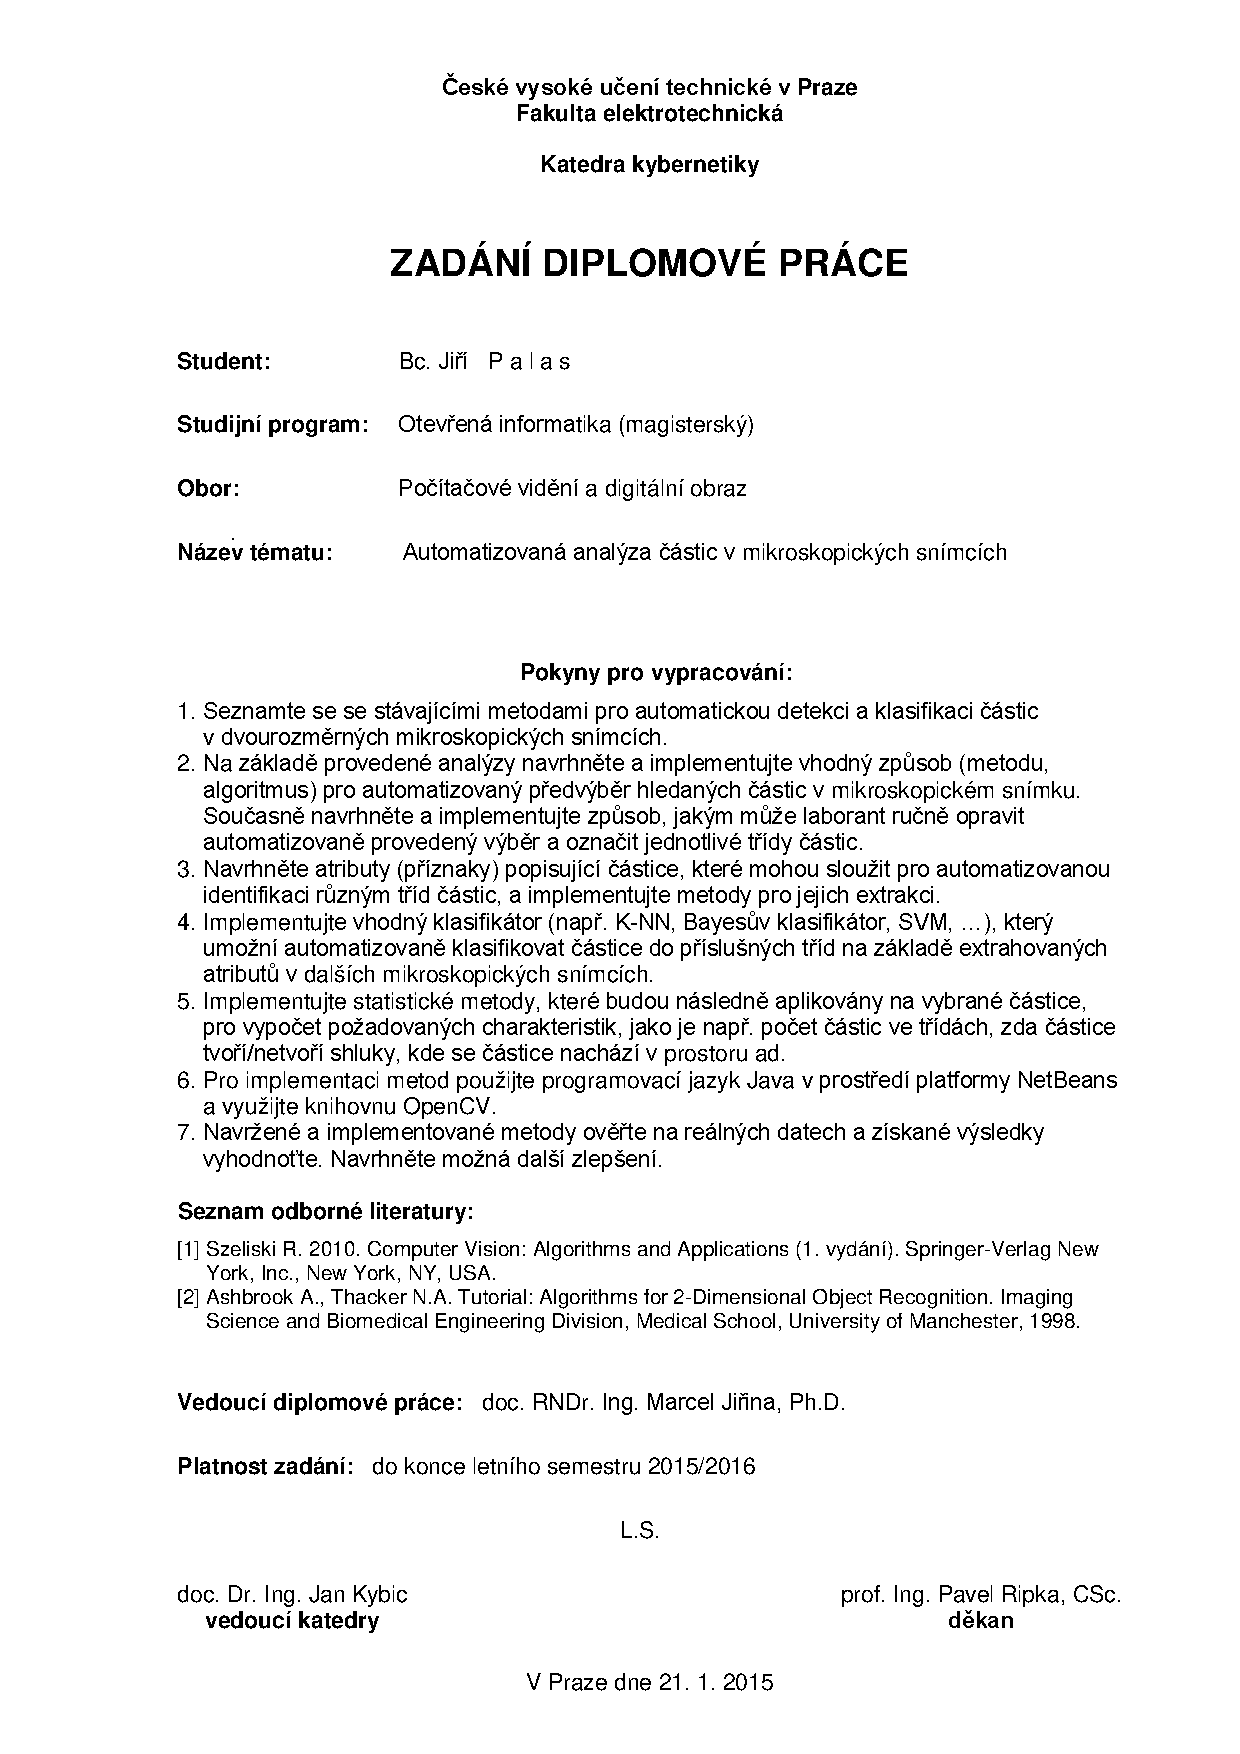
\includepdf[pages={1,{}}]{zadani.pdf}

%%%%%%%%%%%%%%%%%%%%%%%%%%    Titulni stranka / Title page 

\coverpagestarts

%%%%%%%%%%%%%%%%%%%%%%%%%%%    Podekovani / Acknowledgements 

\acknowledgements
\noindent
Na tomto místě bych rád poděkoval mamince za vaření obědů a večeří během krušných hodin psaní.


%%%%%%%%%%%%%%%%%%%%%%%%%%%   Prohlaseni / Declaration 

\declaration{V~Praze dne 11.\,5.\,2015}


%%%%%%%%%%%%%%%%%%%%%%%%%%%%    Abstract 
 
\abstractpage

Abstrakt v angličtině.

% Prace v cestine musi krome abstraktu v anglictine obsahovat i
% abstrakt v cestine.
\vglue60mm

\noindent{\Huge \textbf{Abstrakt}}
\vskip 2.75\baselineskip

\noindent
TODO Ještě nějak lépe přeformulovat

Tato práce si klade za cíl návrh a implementaci software zaměřeného na automatizovanou analýzu částic v mikroskopických snímcích. Práce se zabývá analýzou současných metod zpracování obrazu a strojového učení využitelnými pro automatizovanou detekci, klasifikaci a analýzu mikroskopických částic. Na jejím základě je navržen a implementován algoritmus pro automatizovanou detekci a klasifikaci částic. V rámci práce jsou navrženy a implementovány metody vizuální a interaktivní analýzu detekovaných a klasifikovaných částic.

%******************************  Obsah / Table of Contents 
\tableofcontents

%******************************  Seznam obrazku / List of Figures 
\listoffigures

%******************************  Seznam tabulek / List of Tables
\listoftables

%**************************************************************

\mainbodystarts
% horizontalní mezera mezi dvema odstavci
%\parskip=5pt
%11.12.2008 parskip + tolerance
%\normalfont
\fontsize{11pt}{15pt}\selectfont
\parskip=0.3\baselineskip plus 0.2\baselineskip minus 0.1\baselineskip

% Odsazeni prvniho radku odstavce resi class book (neaplikuje se na prvni 
% odstavce kapitol, sekci, podsekci atd.) Viz usepackage{indentfirst}.
% Chcete-li selektivne zamezit odsazeni 1. radku nektereho odstavce,
% pouzijte prikaz \noindent.


%*****************************************************************************
\chapter*{Úvod}

\section{Motivace}
V současné době se čistý a aplikovaný výzkum v biologii, medicíně a nanotechnologiích opírá o pozorování procesů uvnitř buněk, tkání a orgánů. Mezi takové procesy patří pozorování distribuce léčiv a genů, lokalizaci nádorů, toxikologickému testování, prověřování zdravotních rizik, reakce na chirurgické implantáty atd.~\cite{np:ostrowski}~\cite{np:mayhew}~\cite{np:coloc}.

Pro pozorování těchto procesů se využívají nano-částice (NP). NP jsou částice o rozměrech mezi 1-100~nm. Mezi nejčastěji používané NP patří částice vytvořené chemických sloučenin s kovy. Různé typy NP se odlišují buď tvarem nebo velikostí. Na základě svých vlastností pak NP vykazují specifické chování ve výše zmíněných procesech~\cite{np:intro}.

NP mají velice malý rozměr na to aby se daly snímat pomocí světelné mikroskopie. Proto se k jejich pozorování používají biologické zobrazovací metody pracující ve velikém rozlišení. Mezi takové metody patří například transmisní elektronová mikroskopie (TEM), rastrovací elektronová mikroskopie (SEM) a atd.~\cite{np:ostrowski}~\cite{np:mayhew}~\cite{np:coloc}. Výsledkem těchto zobrazovacích metod je snímek nebo série snímků.

Snímky jsou následně vědci či laboranty vyhodnocovány. Pracovníci UAKČR UMG uvedli, že postrádají kvalitní, specializovaný a přitom jednoduchý nástroj pro vyhodnocování snímků s nanočásticemi.

Tato práce si klade za cíl vytvořit aplikaci pro vyhodnocování snímků. Práce klade důraz na vytvoření co největší úrovně automatizace v aplikaci. Tak aby došlo k celkovému zkvalitnění a zrychlení vyhodnocování jednotlivých snímků. Základem pro vyhodnocování snímků je lokalizace jednotlivých částic. Dále jejich úspěšná klasifikace do jednotlivých tříd (kategorií) podle typů NP. Následná expertní analýza laborantem.

\section{Přehled}
V první kapitole práce definuje požadavky na aplikaci a popisuje data s částicemi.

Ve druhá kapitola se zabývá problémem detekce částic. Nejprve jsou rozebrány možné způsoby jak částice v obraze detekovat. Následně je popsán vybraný algoritmus pro jejich detekci. Nakonec jsou uvedeny výsledky detekce částic na vybraných snímcích.

Třetí kapitola se zabývá problematikou klasifikace částic. Jsou zmíněny jednotlivé přístupy ke klasifikaci. Dále je popsán vybraný klasifikační algoritmus. Nakonec jsou uvedeny výsledky klasifikace částic na vybraných snímcích.

Další kapitola popisuje návrh aplikace uživatelského rozhraní aplikace. Jsou rozebrány její jednotlivé části a jejich jednotlivé části.

Následující kapitola uvádí jak je aplikace realizována.


 




% *****************************************************************************
\chapter{Analýza}
Tato kapitola nejprve popisuje základní definované požadavky na funkčnost aplikace. Dále pak definuje data, se kterými aplikace pracuje. 

\section{Specifikace}
Na základě návštěvy pracoviště UMG jsou popsány požadavky na aplikaci pro automatizovanou analýzu mikroskopických snímků obsahující nanočástice:

Typická práce laboranta vyhodnocujícího NP se sestává z následujících částí:
\begin{itemize}
	\item příprava biologického vzorku
	\item nasnímání vzorku pomocí elektronového mikroskopu
	\item identifikace částic
	\item klasifikace (kategorizace) vzorků
	\item analýza vzorku
\end{itemize}
Práce se zaměřuje na automatizaci nebo částečnou automatizaci bodů 3-5. Ty se pak podrobněji zahrnují
\begin{itemize}
	\item načítání mikroskopické obrázky ve formátech TIFF, JPEG
	\item zobrazení načtených obrázků
	\item schopnost detekovat NP v obrázku
	\item schopnost nalézt těžiště NP
	\item zobrazení detekovaných NP v obrázku
	\item možnost označit jednotlivé třídy NP
	\item automatizace označování NP
	\item vizuální shluková analýza NP
\end{itemize}

\section{Data}

\begin{figure}
\centering
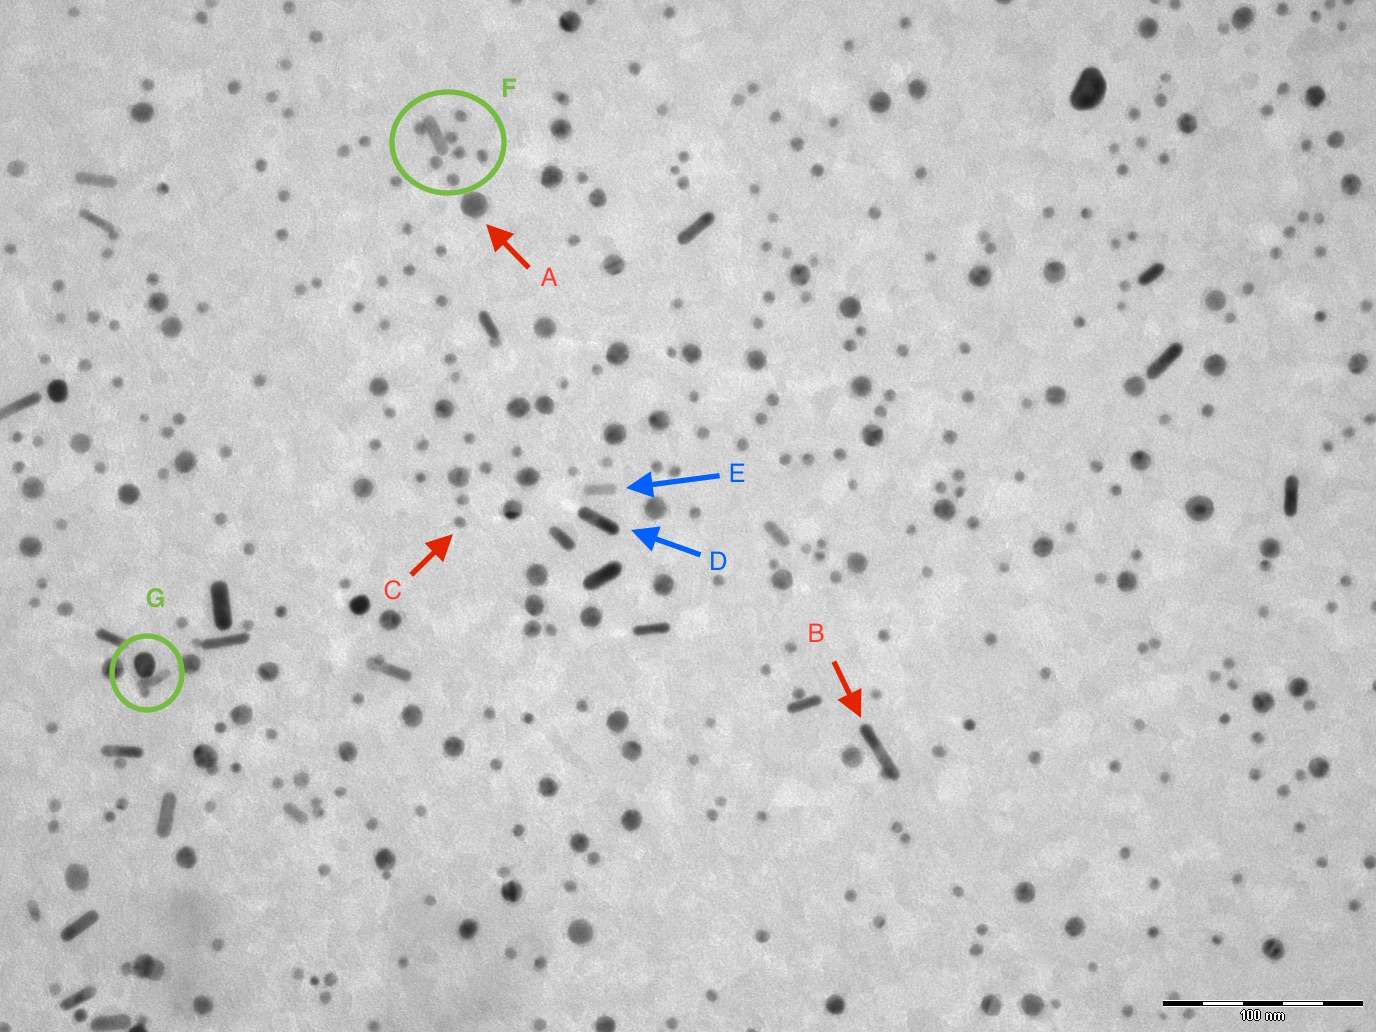
\includegraphics[scale=0.3]{figures/data1.jpg}
\caption[Příklad vyhodnocovaného snímku.]{Příklad vyhodnocovaného snímku. Červené šipky ukazují různé tvary vyhodnocovaných NP. Tvar A: Koláč. Tvar B: Tyčinka. Tvar C: Kolečko. Částice E a D demonstrují možné rozdíly v jasech částic. Region G zobrazuje příklad překryvu částic. Region F zobrazuje příklad shlukování částic.}
\label{fig:data_example}
\end{figure}

Aplikace se zabývá vyhodnocováním NP obsažených ve snímcích jako na obr. \ref{fig:data_example}. Snímky jsou 8-bitové jednokanálové (šedotónové) obrázky s rozlišením mezi 2 a 3 megapixely.

Částice ve snímku můžeme pozorovat jako kontrastní útvary s nízkým jasem (tmavě šedé až černé) na světlém pozadí.

Snímané vzorky jsou v mikroskopu nerovnoměrně osvětleny. To se projevuje na nerovnoměrném rozložení jasu v obrázku. Viz. levý horní roh a pravý horní roh na obr.~\ref{fig:data_example}. Dalším negativním jevem, který znesnadňuje detekci je tendence NP tvořit shluky viz. region F na obr.~\ref{fig:data_example} a překrývat se viz. region G na obr.~\ref{fig:data_example}. Navíc ani částice nemají jednotnou úroveň jasu viz. částice E a D na obr.~\ref{fig:data_example}.

Práce rozlišuje tři typy částic A, B, C viz. obr.~\ref{fig:data_example}. Pracovní názvy těchto částic jsou koláč (A), tyčinka (B) a kolečko (C). K rozlišení těchto částic uvažujeme informaci o tvaru a velikosti. Jednotlivé částice lze považovat za konvexní útvary \cite{art:np_convex}. NP mohou být v obrázku libovolně orientované.  V určitých částech snímku splývají s pozadím více viz. a v některých méně viz. Částice nemají výraznou texturu. Snímek typicky obsahuje 300 - 700 částic.

Na základě provedené charakteristiky obrazu a částic je vybrán vhodný detekční a klasifikační algoritmus viz kapitola \ref{sec:detekce} a kapitola \ref{sec:klasifikace}.

%%% Detekce nanočástic %%%%%%%%%%%%%%

\chapter{Detekce nanočástic}
\label{sec:detekce}
Tato kapitola se zabývá problematikou segmentace nanočástic z jednotlivých snímků.

\subsection{Úvod do problematiky}

Cílem detekčního algoritmu je úspěšně nalézt jednotlivé částice v obraze. Dále je třeba nalezené částice popsat modelem na jehož základě bude částice možné klasifikovat pomocí klasifikačního algoritmu a dále vyhodnocovat.

Pro úspěšnou detekci částic je nejprve potřeba jejich segmentace. Segmentace je proces při kterém jsou ze snímku odděleny jednotlivé objekty a části od pozadí. Jedná se často o nejsložitější a nejdůležitější krok při analýze obrazu.

Navzdory důležitosti, existuje pouze limitované množství zdrojů o automatické segmentaci nanočástic využitelných pro náš případ. Všechny nalezené zdroje se zabývají převážně detekcí NP kruhovitého tvaru \cite{art:mcfarland}\cite{art:glotov}\cite{art:chen}. Na druhou stranu ale existuje rozsáhlý výzkum zabývající se segmentací biologických buněk. V následujícím textu je shrnuta literatura zabývající se segmentací biologických buněk. Tento směr výzkumu je přímo spjat s jedním z cílů této práce \cite{art:ultimate}.

Velice často používanou metodou pro segmentaci buněk je je prahování založené na charakteristikách histogramu obrázku. Přehled prahovacích technik uvádí \cite{art:sahoo88}. Pro obdržení uspokojivého výsledku segmentace za pomoci prahování je ale zapotřebí pozadí obrázku s neměnnou intenzitou. Je také třeba pamatovat na to, že malá změna v úrovni prahu může mít negativní dopad na na další analýzu obrázku \cite{art:wahlby}.

\textbf{Adaptivní prahování} nebo také lokální automatické prahování může být řešení pro prahování obrázku ve kterém intezita pozadí kolísá. Tato metoda ale stále neřeší problémy spojené s segementací objektů které tvoří shluky. Prahování nemusí být finálním krokem v segmentačním procesu. Naopak často bývá využíván právě jako první krok před dalším zpracování např. pomocí morfologických operací \cite{book:imgproc_gonzalez} \cite{art:wahlby}.

Další hojně užívanou metodou pro segmentaci buněk je tzv.~\textbf{watershed} a jeho odvozeniny. Metoda nejprve nalezne body (markery) ukazující přibližnou polohu buněk a následně segmentuje obrázek na několik oblastí ovlivněných markery~\cite{art:watershed1} \cite{art:watershed2}\cite{art:watershed3}\cite{art:wahlby}.

\textbf{Graph-cut} metody jsou také aplikovány na segmentaci buněk. Metoda zkonstruuje graf z obrázku kde každý pixel odpovídá jednotlivým vrcholům grafu. Každý pár vrcholů je spojen se sousedními vrcholy hranou jejíž váha odpovídá podobnosti intenzit sousedních pixelů. Segmentace pak hledá normalizovaný minimální řez grafem \cite{art:grabcut1}. Avšak tento přístup špatně separuje překrývající se buňky, obzvláště pokud je jejich intenzita podobná. Existuje úprava která tento problém řeší, funguje však pouze na částice buňky kruhového tvaru \cite{art:ultimate}.

Mezi další segmentační metody použivané při segmentaci buněk se řadí \textbf{aktivní kontury} \cite{art:active_contours1} \cite{art:active_contours2}. Aktivní kontury jsou originálně navržené k segmentaci jednoho objektu s komplikovaným tvarem. Avšak po úpravě vícefázový algorimus může být použit k segmentaci více nepřekrývajících se objektů. Článek \cite{art:ultimate} na základě dalších použití na segmentaci překrývajících se buněk nedoporučuje.

\subsection{Popis použitého řešení}

Na základě předchozí analýzy byla ozkoušena segmentace metodami prahování \textit{watershed} a adaptivního prahování.

Adaptivní prahování překvapivě produkuje od začátku dobrou míru segmentace. Avšak nedokáže oddělit částice, které se dotýkají nebo překrývají. Proběhl pokus zpřesnit výsledky pomocí watershed algoritmu. Avšak výsledek ke zpřesnění výstupu segmentace nedošlo, protože nebyl nalezen korektní způsob umístění markerů. Bylo vyzkoušeno umístění na základě distanční transformace \cite{opencv:watertut} a na základě \textit{ultimátní eroze pro konvexní sety } \cite{art:ultimate}. Současné řešení se tedy ustálilo na níže popsaném řešení.

Snímky s NP obsahují malé množství šumu, proto je obrázek předzpracován mediánového filtru s oknem o velikosti $3x3$ pixely. 

Z důvodů problémů s jasem popsaných dříve je pro úvodní segmentaci vybrán algoritmus lokálního adaptivního prahování. Algoritmus volí práh pro každý pixel individuálně na základě rozsahu hodnot intenzity v lokálním okolí \cite{on:adaptive}. Výstupem algoritmu je pak binární obrázek.

V této aplikaci se hodnota prahu v bodě $(x,y)$ získává jako:
\begin{equation}
t(x,y) = \sum_{i=x-(B-1)/2}^{x+(B-1)/2} \sum_{j=y-(B-1)/2}^{y+(B-1)/2}f(i,j) - C
\end{equation}
Kde $t(x,y)$ je hodnota prahu v bodě $(x,y)$, $f(i,j)$ hodnota intenzity v bodě $(i,j)$, $B$ velikost okna a $C$ konstanta. Velikost okna musí být liché číslo.

Binární obrázek získaný prahováním je následně upraven pomocí morfologické operace \textit{otevření} s jádrem:
\begin{equation}
\begin{bmatrix}
1 & 1 & 1 \\
1 & 1 & 1 \\
1 & 1 & 1 \\
\end{bmatrix}
\end{equation}

V binarní obrázek, upraveným morfologickou operací jsou následně prostřednictvím algoritmu \cite{suzuki85} nalezeny obrysy jednotlivých NP. Obrys je reprezentován vektorem bodů, kterého ho tvoří.

K detekci byla využita implementace adaptivní filtrace a algoritmu \cite{suzuki85} z OpenCV\cite{opencv_library}. Adaptivní filtrace využívá funkce \textit{adaptiveThresh} a algoritmus na vyhledávání obrysů pak funkci \textit{findContours}.

\subsection{Výsledky segmentace}
Segmentace a její vyhodnocení výsledků probíhalo na datech snímcích pocházejících z UMG. Ze snímků které jsou k dispozici je zvoleno 7 mikroskopických snímků obsahujících variující tvary částic.Ve vzorcích 1, 2, 7 se vyznačují malou mírou shlukování částic. Naopak ve vzorcích 3, 4, 5, 6 jsou částice poskládány blíže sobě a některé se překrývají.

Výstupy segmentace algoritmu jsou prezentovány pomocí barevného značení, kde kontura nalezené částice je zobrazena červeně.

\begin{figure}[ht]
	\centering
	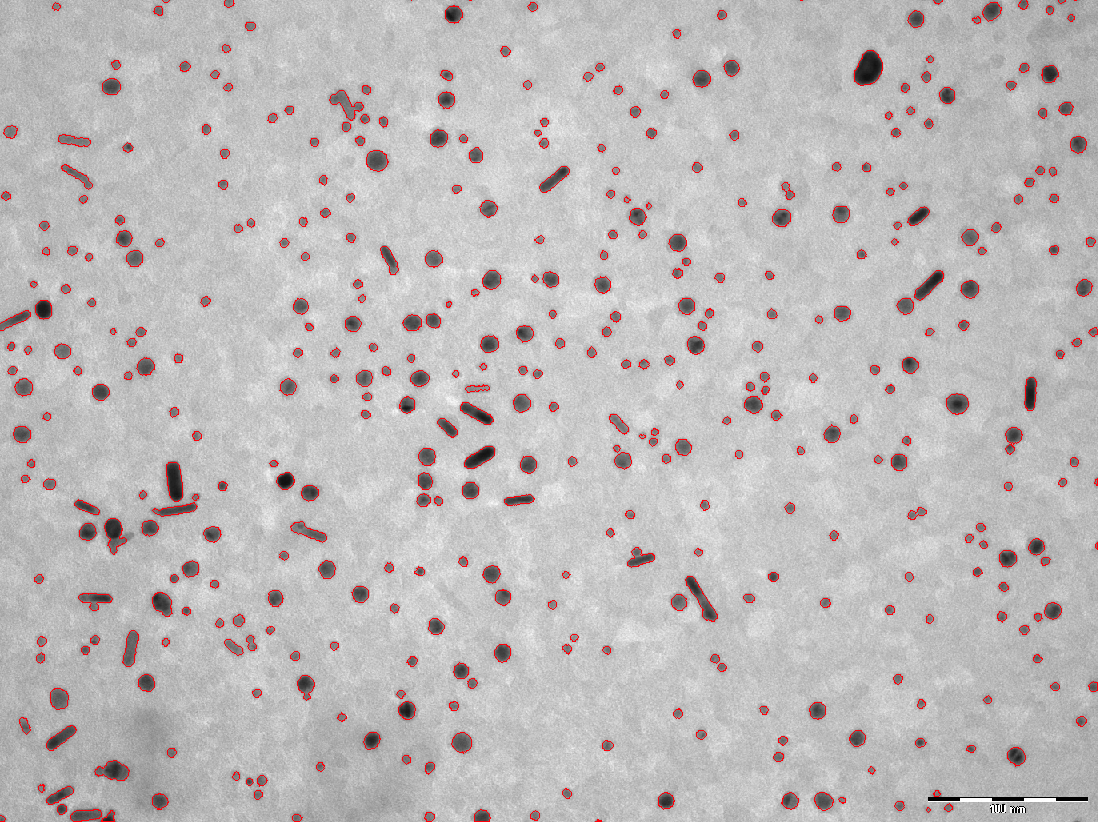
\includegraphics[width=\textwidth]{figures/segment_result.png}	
	\caption{Příklad výstupu segmentačního algoritmu na vzorku 5.}
	\label{fig:segment_result}
\end{figure}

Příklad výstupu segmentačního algoritmu je možné pozorovat na obr.~\ref{fig:segment_result}. Detaily chybně provedené segmentace jsou znázorněny na obr.~\ref{fig:segment_problems}. 

Vyhodnocení výstupu segmentace je možné pozorovat v tabulce \ref{tab:segment_results}. Nejčastějším problémem při segmentaci je segmentace spojených částic typu tyčinka a kolečko.  

\begin{figure}[ht]
	\begin{center}
	\begin{subfigure}[l]{0.45\textwidth}
		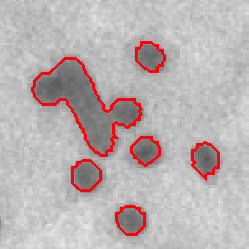
\includegraphics[scale=1]{figures/segment_problem1.png}
	\end{subfigure}
	~
	\begin{subfigure}[r]{0.45\textwidth}
		\begin{subfigure}[b]{\textwidth}
			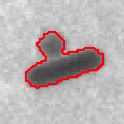
\includegraphics[scale=1]{figures/segment_problem2.png}
		\end{subfigure}
	
		\begin{subfigure}[b]{\textwidth}
			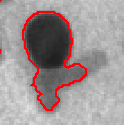
\includegraphics[scale=1]{figures/segment_problem3.png}
		\end{subfigure}
	\end{subfigure}
	\end{center}
	\caption{Příklady chybně provedené segmentace.}
	\label{fig:segment_problems}
\end{figure}

\begin{table}[htp]
\centering
\begin{tabular}{|l|l|l|l|}
\hline
\rowcolor[HTML]{C0C0C0} 
Vzorek & Chybná segmentace & Očekáváno & Přesnost \\ \hline
1      & 1                 & 353       & 0.997    \\ \hline
2      & 1                 & 383       & 0.997    \\ \hline
3      & 29                & 435       & 0.932    \\ \hline
4      & 31                & 458       & 0.932    \\ \hline
5      & 27                & 426       & 0.936    \\ \hline
6      & 8                 & 411       & 0.980    \\ \hline
7      & 1                 & 338       & 0.997    \\ \hline
Celkem & 98                & 2809      & 0.965    \\ \hline
\end{tabular}
\caption{Výsledky segmentace.}
\label{tab:segment_results}
\end{table}

\chapter{Klasifikace}
\label{sec:klasifikace}
Tato kapitola se se zabývá problematikou klasifikace detekovaných částic. V úvodu kapitoly je rozvedena problematika klasifikace a uvedeny metody strojového učení, které je možné využít při řešení této problematiky. Následně je rozveden přístup pro klasifikaci částic do jednotlivých tříd A, B nebo C, použitý v aplikaci  V závěru kapitoly pak jsou uvedeny jednotlivé výsledky klasifikace pomocí zvoleného K-NN klasifikátoru.

\subsection{Úvod do problematiky}
Klasifikace je jedním z nejčastějších problémů se kterými se člověk setkává. Klasifikační problém se objevuje vždy, když určitý objekt potřebuje být začleněn do předdefinované skupiny \cite{art:neural_networks}.

Mezi metody, které řeší klasifikační problémy patří metody strojového učení. V biologii bylo strojové učení již aplikováno na řadu problému v oblastech vývoje léků \cite{art:machine1}, analýza sekvencí DNA \cite{art:machine2}, proteomika \cite{art:machine3} a další. Mimo biologii se strojové učení využívá např. pro rozpoznávání textu, obličejů atd. Metody strojového učení dělíme na dvě skupiny, učení bez učitele a učení s učitelem.

První skupinou jsou metody tzv. \textit{učení bez učitele}. Tyto metody se obvykle využívají při zkoumání dat o kterých máme málo informací nebo nedokážeme vytvořit trénovací metody. Cílem učení bez učitele je spojovat skupiny dat do shluků na základě měření podobnosti nebo usnadnění následného vytěžování dat redukcí jejich dimensionality.

Druhou skupinu tvoří tvz. \textit{metody učení s učitelem}. V tomto přístupu, uživatelé generují, z celé sady dat, data trénovací pomocí anotace reprezentativních vzorků. Anotaci dat se rozumí přiřazení vzorku do skupiny. Na základě těchto trénovacích dat je poté algoritmus strojového učení schopen podle definovaných pravidel a postupů zařadit do jednotlivých tříd i dosud neznámé vzorky dat.

Protože jednotlivé částice jsou klasifikovány na základě anotací poskytnutých laborantem jsou nadále uvažovány pouze metody strojového učení s učitelem.

Jak bylo řečeno ve strojovém učení s učitelem, člověk, jako expert, nejprve definuje trénovací data anotováním vybraných příkladů z celkové množiny dat. V našem případě tvoří množinu všech dat detekované částice z jednoho či několika snímků. Trénovací množina je pak vybírána z této množiny anotováním jednotlivých částic. Ve strojovém učení proces trénování slouží k získání vnitřních parametrů klasifikačního modelu na jejichž základě jsou pak jednotlivé příklady klasifikovány.

Mezi současné klasifikační algoritmy učení s učitelem patří např. rozhodovací stromy, Support Vector Machine (SVM), naivní Bayes, AdaBoost, neuronové sítě nebo algoritmus k-nejbližších sousedů (K-NN) a další ~\cite{book:pattern_class}.

Bayesovská rozhodovací metodika spoléhá na statistický pravděpodobnostní model. Podle tohoto modelu je pak určena jednotlivá příslušnost instancí do tříd \cite{art:neural_networks}.

Metoda \textit{rozhodovacích stromů} je založena na víceúrovňovém rozhodování. Spočívá na principu kdy je komplexní rozhodovací problém rozložen na více jednodušších rozhodovacích problémů na jednotlivých úrovních \cite{art:decision_trees}. 

Support vector machines (SVM) je metoda která se snaží nalézt dělící nadrovinu, která rozdělí data rozdílných tříd, tak aby vzdálenost nejbližších trénovacích příkladů z různých tříd byla co největší. Protože data různých tříd nemusí být vždy oddělitelná pomocí nadroviny většina implemtací SVM je založena na \textit{měkkém okraji} (soft-margin), který umožňuje špatnou klasifikaci. Špatně klasifikované příklady jsou pak váženy cenovou funkcí. SVM je robustní na příznaky s vysokým podílem šumu \cite{art:machine_in_cell}.

Adaptive bootsing (AdaBoost) je založen na kombinaci několika slabých klasifikátorů k formování silného klasifikátoru iterativním přidáváním a vážením jednotlivých slabých klasifikátorů. Příkladem slabého klasifikátoru může být např. prahová funkce. Nevýhodou AdaBoostu je náchylnost na data s vysokým podílem šumu a tzv. \textit{outlierů}.

Neuronové sítě je skupina algoritmů inspirovanými neuronovými spojeními v lidském mozku. Skládá se z umělých neuronů, jejichž inspirace pochází právě z biologických neuronů. Jednotlivé neurony jsou navzájem propojeny a navzájem si předávají signály, které se transformují pomocí přenosových funkcí. Neuron může mít mnoho vstupů ale pouze jeden výstup. Příkladem neuronu může být např. perceptron~\cite{art:neural_networks}. 

Typické kroky při tvorbě klasifikátoru učení s učitelem jsou:
\begin{itemize}
\item Určení trénovací množiny dat
\item Zisk trénovací množiny dat
\item Tvorba příznaků
\item Volba trénovacího algoritmu
\item Vyhodnocení výsledků
\end{itemize}

\section{Trénovací množina a volba příznaků}
Trénovací množinu dat tvoří laborantem anotované částice s přiřazenou příslušností do A, B nebo C. Částice jsou získávány jako výstup detekčního algoritmu. Anotaci a výběr trénovací množiny pak zajistí laborant skrze rozhraní aplikace.

Jednotlivé částice od sebe odlišujeme tvarem, definovaným vektorem bodů, a velikostí plochy v pixelech. Tyto dva příznaky použijeme k zformování vektoru příznaků na který budeme aplikovat klasifikační algoritmus.

\section{Volba klasifikačního algoritmu}

Na základě malého počtu příznaků, tvaru prostoru příznaků a průběžných experimentálních výsledků byl ke klasifikaci je vybrán algoritmus \textbf{k-nejbližších sousedů (K-NN)}.

K-nejbližších sousedů (K-NN) je neparametrická metoda využívaná pro klasifikaci a regresi. Spočívá ve vyhledávání k nejbližších sousedů v prostoru příznaků. K-NN potřebuje pro svou funkci definovat funkci vzdálenosti. Existuje řada metrik jak vzdálenost měřit. Mezi takové metriky patří např. Minkowského metrika také uváděná jako $L_{k}$ norma. Její podmnožiny tvoří např. Manhattanská či Eukleidovská vzdálenost \cite{book:pattern_class}.

Práce využívá pro měření vzdálenosti eukleidovský metriku na vektor o dvou příznacích. Prvním příznakem je plocha částice a druhým tvarová podobnost.

Tvarovou podobnost částice porovnáváme na základě Hu-momentů\citep{art:hu_moments}. Jedná se o momenty pomocí nichž dokážeme tvar identifikovat. Výsledkem je deskriptor invariantní vůči translaci, rotaci z změně měřítka. Moment tvaru v binárním obrázku o rozměrech M x N je popsán jako:
\begin{equation}
u_{pq} = \sum^{N-1}_{j=0}\sum^{M-1}_{i=0} i^p j^q f(i,j)
\label{eq:moment}
\end{equation}
Kde $f(x,y)$ je intenzita pixelu (v binárním obrázku 1 nebo 0) na souřadnicích $(x,y)$ a $p+q$ udává stupeň momentu.

Protože výpočet momentu je funkce vzdálenosti mezi pixely tvaru a středem všech měření vztaženými relativně k těžišti tvaru $(x^\prime, y^\prime)$  za účelem odstranění stupně volnosti v posuvu. Souřadnice těžiště pak lze vypočítat za použití rovnice \ref{eq:moment} jako:
\begin{equation}
i^\prime = \frac{u_{10}}{u_{00}} \,\,\,\,\, j^\prime = \frac{u_{01}}{u_{00}}
\end{equation}
Odtud pak relativní momenty:
\begin{equation}
u_{pq} = \sum^{N-1}_{j=0}\sum^{M-1}_{i=0} (i^\prime - i)^p (j^\prime -j)^q f(i,j)
\end{equation}
Jednotlivé momenty nejsou samy o sobě dostatečně popisné aby dokázaly reprezentovat libovolné tvary, nebo udržovaly invariantní charakteristiky tvaru. Na jejich základě je odvozeno sedm invariantních momentových funkcí jejichž forma je již v hodná pro reprezentaci tvaru. Tyto momenty jsou:

\begin{equation}
m_1 = (u_{20} + u_{02})
\label{eq:hu1}
\end{equation}
\begin{equation}
m_2 = (u_{20} - u_{02})^2 + 4u^2_{11}
\end{equation}
\begin{equation}
m_3 = (u_{30} - 3u_{12})^2 + (3u_{21} - u_{30})^2
\end{equation}
\begin{equation}
m_4 = (u_{30} + u_{12})^2 + (u_{21} + u_{03})^2
\end{equation}
\begin{equation}
\begin{split}
m_5 = (u_{30} - 3u_{12})(u_{30} + u_{12})((u_{30} + u_{12})^2 - 3(u_{21} + u_{03})^2)\\
+ (3u_{21} - u_{03})(u_{21} + u_{03}) (3(u_{30} + u_{12})^2 - (u_{21} + u_{03})^2)
\end{split}
\end{equation}
\begin{equation}
\begin{split}
m_6 = (u_{20} - u_{02}) - (u_{30} + u_{12})^2 - (u_{21} + u_{03})^2 \\
+ 4u_{11}(u_{30} + 3u_{12})(u_{21} + u{03})
\end{split}
\end{equation}
\begin{equation}
\begin{split}
m_7 = (3u_{21} - u_{03})(u_{30} + u_{12}) ((u_{30} + u_{12})^2 - 3(u_{21} + u_{03})^2)\\
- (u_{30} - 3u_{12})(u_{21} + u_{03})(3(u_{30} + u_{12})^2 - (u_{21} + u_{03})^2)
\end{split}
\label{eq:hu7}
\end{equation}

Podobnost jednoho tvaru s druhým pak vypočítáme jako:
\begin{equation}
s(A,B) = \sum_{i=1\cdots 7}\vert m_i^A - m_i^B\vert
\label{eq:shape_similarity}
\end{equation}
Kde $s(A,B)$ je podobnost tvarů A a B, $m_i$ je jeden ze sedmi Hu-momentů z rovnic \ref{eq:hu1}-\ref{eq:hu7}. Výsledkem je hodnota rostoucí od $0$ a platí, že čím větší menší podobnost tím větší hodnota.

Jeden z hlavních nedostatků K-NN při výpočtu vzdálenosti od trénovacích dat je příklad kdy jednotlivé příznaky mají rozdílné škály nebo pokud se jedná o směs numerických a kategorických hodnot. Toto je příklad mnou zvolených příznaků. Velikost plochy částic se pohybuje mezi desítkami až stovkami pixelů. Zatímco podobnost se pohybuje v přibližném rozpětí mezi 0 a 2. Hodnoty je proto třeba normalizovat. Jinak by klasifikátor klasifikoval částice pouze podle velikosti \cite{flusser2000} \cite{art:objrec2d}.

Každý příznak $x_ij (i = 1\cdots k, j = 1\cdots n)$, kde $k$ je velikost vektoru příznaků a $n$ velikost trénovací množiny, je pak normalizován jako:
\begin{equation}
x^\prime_{ij} = \frac{x_ij - min_i}{max_i - min_i}
\end{equation}
Kde $min_i = \min\limits_{i=1\cdots k}(x_{ij})$ a $max_i = \min\limits_{j=1\cdots k}(x_{ij})$.

Normalizace se provádí vždy při přidání nové částice mezi trénovací data. V případě, že příznaky nově přidané částice posouvají $min_i$ nebo $max_i$ jsou přeškálovány i ostatní hodnoty podle nového rozpětí.

Originální prostor, ve kterém modely jednotlivých částic existují je více-dimenzionální. Z tohoto důvodu je originální prostor špatně zobrazitelný. Můžeme ale zobrazit transformovaný prostor příznaků pro jednotlivé částice viz. grafy na obr.~\ref{fig:feature_space_tycinka}, ~\ref{fig:feature_space_kolac},~\ref{fig:feature_space_kolecko}.

\begin{figure}[H]
	\centering
	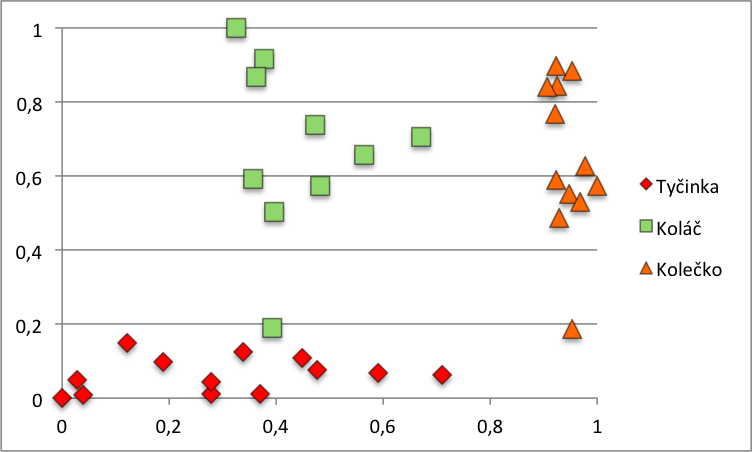
\includegraphics[height=0.3\textheight]{figures/feature_space_tycinka.png}
	\caption{Prostor příznaků pro částici, která by byla klasifikována jako typ tyčinka. Osa x: rozdíl ve velikostech částic. Osa y: tvarová podobnost. }
	\label{fig:feature_space_tycinka}
\end{figure}
~
\begin{figure}[H]
	\centering
	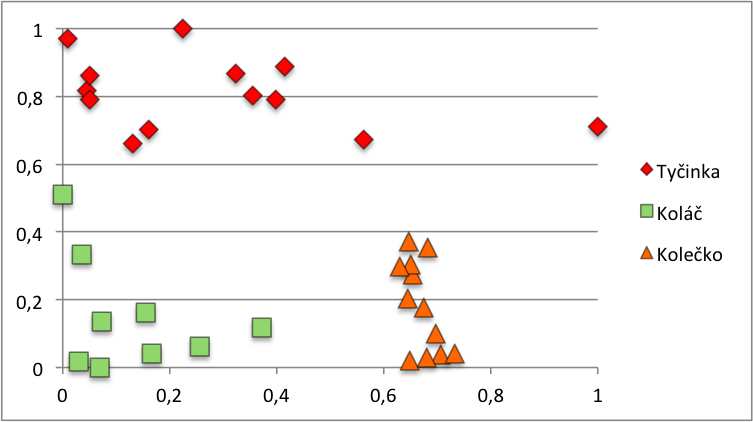
\includegraphics[height=0.3\textheight]{figures/feature_space_kolac.png}
	
	\caption{Prostor příznaků pro částici, která by byla klasifikována jako typ tyčinka. Osa x: rozdíl ve velikostech částic. Osa y: tvarová podobnost.}
	\label{fig:feature_space_kolac}
\end{figure}
~
\begin{figure}[H]
	\centering
	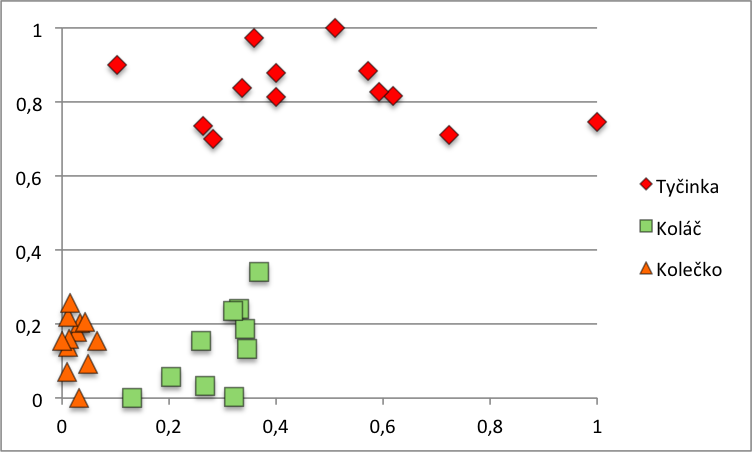
\includegraphics[height=0.3\textheight]{figures/feature_space_kolecko.png}
	\caption{Prostor příznaků pro částici, která by byla klasifikována jako typ kolečko. Osa x: rozdíl ve velikostech částic. Osa y: tvarová podobnost.}
	\label{fig:feature_space_kolecko}
\end{figure}


Souřadnice $x_i$ v transformovaném prostoru vypočítáme jako:
\begin{equation}
x_i = \vert S - S_i \vert
\end{equation}
Kde $i=1 \cdots N$ ($N$ udává velikost trénovací množiny), $S$ plochu testované částice, $S_i$ plochu trénovací částice $i$.

Souřadnici $y_i$ pak udává tvarovou podobnost mezi testovanou částicí a porovnávanou trénovací částicí viz rovnice~\ref{eq:shape_similarity}.

Z grafů je pozorovatelné, že jednotlivé typy částic jsou od sebe výrazně odděleny. Na tomto základě byla vybrána metoda K-NN.

Pro výpočet podobnosti tvarů byla využita funkce \textit{matchShapes} z OpenCV\cite{opencv_library}.

\FloatBarrier
\section{Výsledky klasifikace}

\subsection{Vstupní data}
Trénování a vyhodnocení výsledků probíhalo na datech snímcích pocházejících z UMG. K dispozici je 7 mikroskopických snímků obsahujících variující tvary nanočástic. Výstupy klasifikačního algoritmu jsou prezentovány pomocí barevného značení, kde oražová barva značí částici typu kolečko, červená částici typu tyčinka a žlutozelená typ koláč. 

Výstup automatické klasifikace je porovnáván vůči výstupu jak by částice klasifikoval laborant.

\begin{figure}[hp]
	\centering
	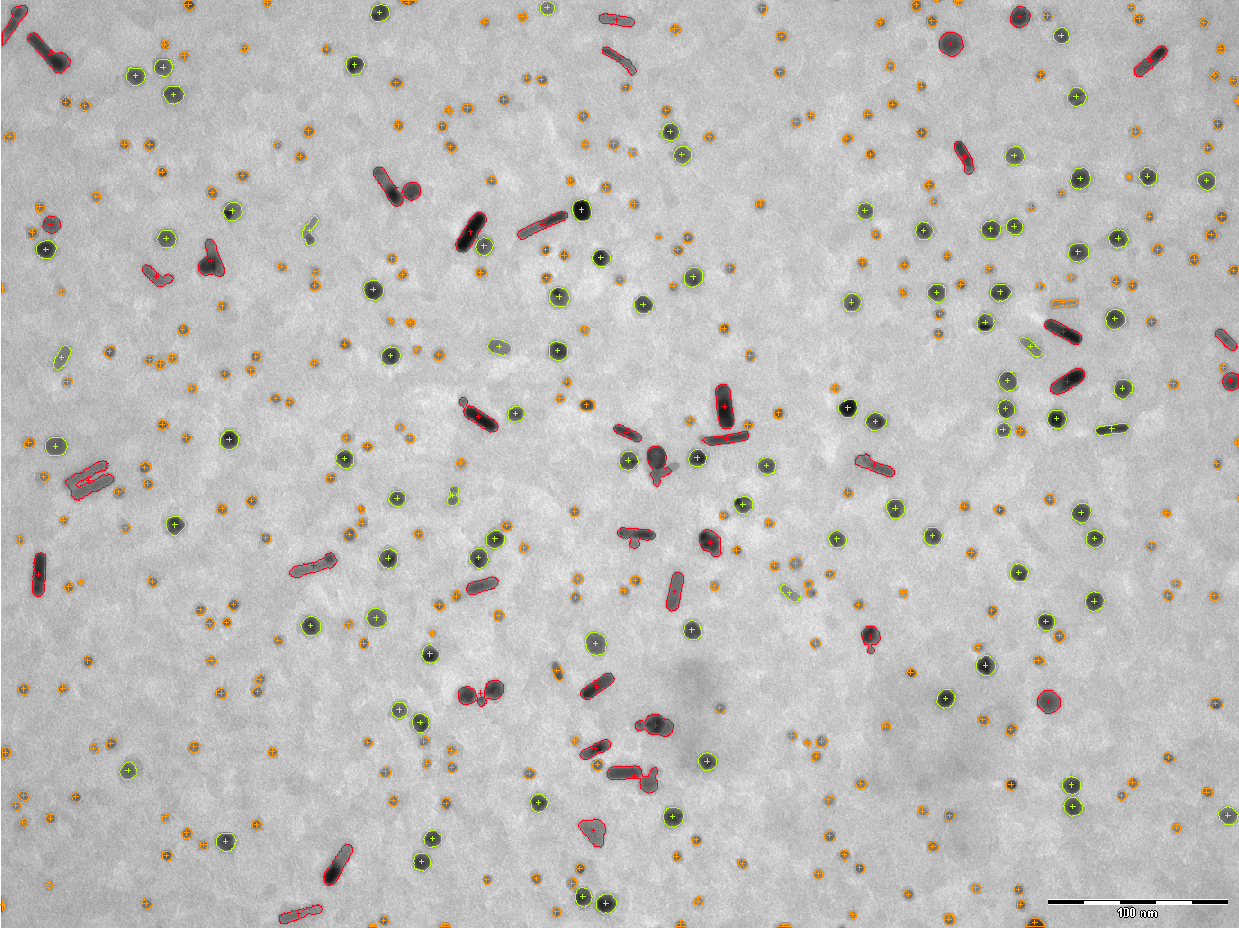
\includegraphics[width=0.85\textwidth]{figures/multi5_klasifikace.png}
	\caption{Množina trénovacích dat.}
	\label{fig:class_input}
\end{figure}

Vstupní trénovací množina je zobrazena na obr.~\ref{fig:class_input}.

Nastavení parametrů:
\begin{itemize}
	\item Velikost okna: 51
	\item C: 21
	\item K: 5 
\end{itemize}

\newpage
\FloatBarrier
\subsection{Vzorek 1}
V této části se nachází zjištěné hodnoty výsledků klasifikace pro vzorek 1.

\begin{figure}[h!]
\begin{center}
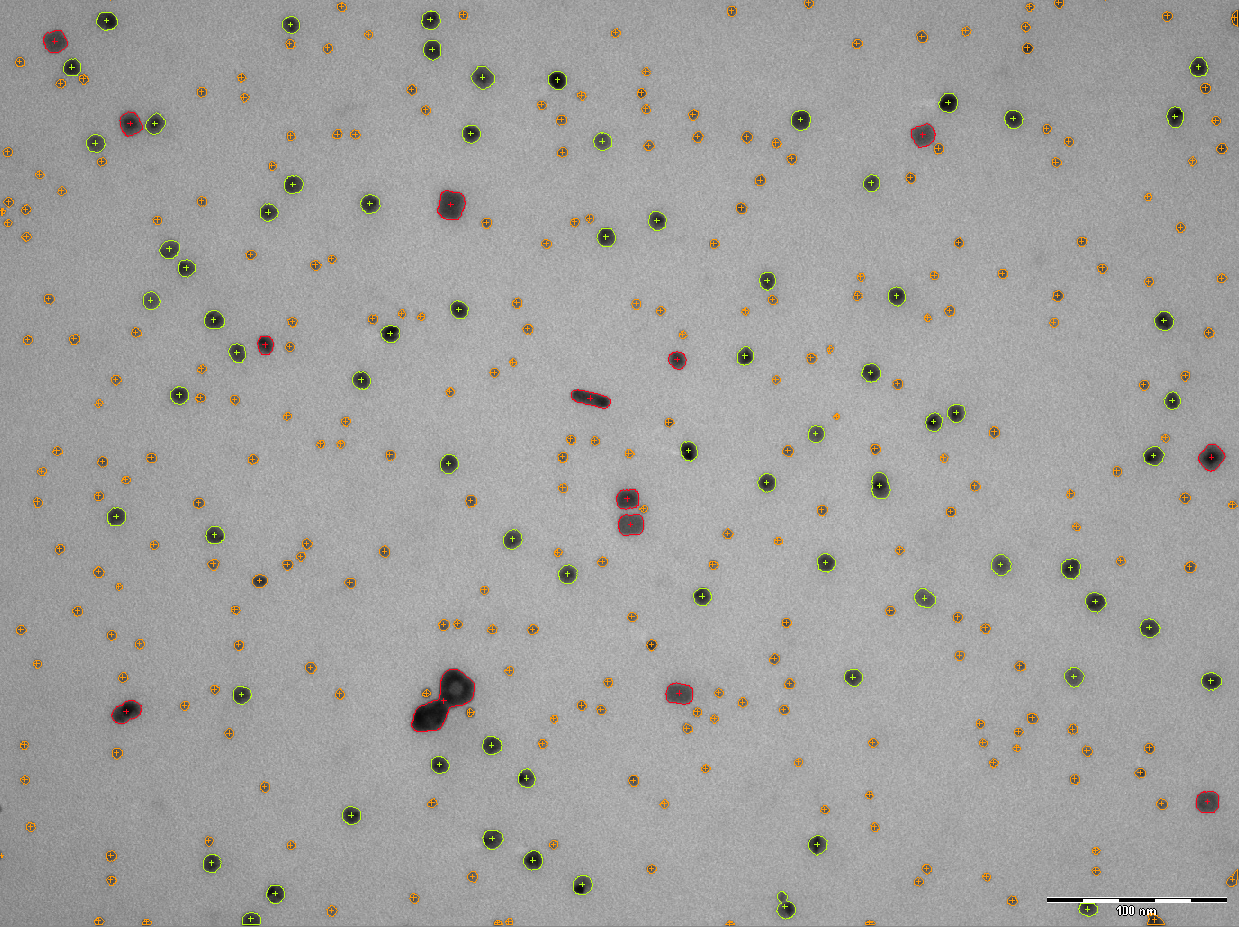
\includegraphics[width=\textwidth]{figures/multi1_klasifikace.png}
\end{center}
\label{fig:class1}
\caption{Výsledek klasifikace částic pro vzorek 1.}
\end{figure}

\begin{table}[h!]
\begin{center}
\begin{tabular}{lllll}
\hline
\rowcolor[HTML]{9B9B9B} 
\multicolumn{1}{|l|}{\cellcolor[HTML]{9B9B9B}Třída} & \multicolumn{1}{l|}{\cellcolor[HTML]{9B9B9B}Dobře} & \multicolumn{1}{l|}{\cellcolor[HTML]{9B9B9B}Špatně} & \multicolumn{1}{l|}{\cellcolor[HTML]{9B9B9B}Celkem} & \multicolumn{1}{l|}{\cellcolor[HTML]{9B9B9B}Přesnost} \\ \hline
\multicolumn{1}{|l|}{-1}                            & \multicolumn{1}{l|}{0}                             & \multicolumn{1}{l|}{2}                               & \multicolumn{1}{l|}{2}                              & \multicolumn{1}{l|}{0,000}                            \\ \hline
\multicolumn{1}{|l|}{0}                             & \multicolumn{1}{l|}{2}                             & \multicolumn{1}{l|}{0}                               & \multicolumn{1}{l|}{2}                              & \multicolumn{1}{l|}{100,000}                          \\ \hline
\multicolumn{1}{|l|}{1}                             & \multicolumn{1}{l|}{267}                           & \multicolumn{1}{l|}{0}                               & \multicolumn{1}{l|}{267}                            & \multicolumn{1}{l|}{100,000}                          \\ \hline
\multicolumn{1}{|l|}{2}                             & \multicolumn{1}{l|}{72}                            & \multicolumn{1}{l|}{11}                              & \multicolumn{1}{l|}{83}                             & \multicolumn{1}{l|}{86,747}                           \\ \hline
\multicolumn{1}{|l|}{Celkem}                        & \multicolumn{1}{l|}{341}                           & \multicolumn{1}{l|}{11}                              & \multicolumn{1}{l|}{352}                            & \multicolumn{1}{l|}{96,875}                           \\ \hline
\end{tabular}
\end{center}
\caption{Vyhodnocení klasifikace částic pro vzorek 1.}
\label{tab:classresult1}
\end{table}

\newpage
\FloatBarrier
\subsection{Vzorek 2}
V této části se nachází zjištěné hodnoty výsledků klasifikace pro vzorek 2.
\begin{figure}[h!]
\center
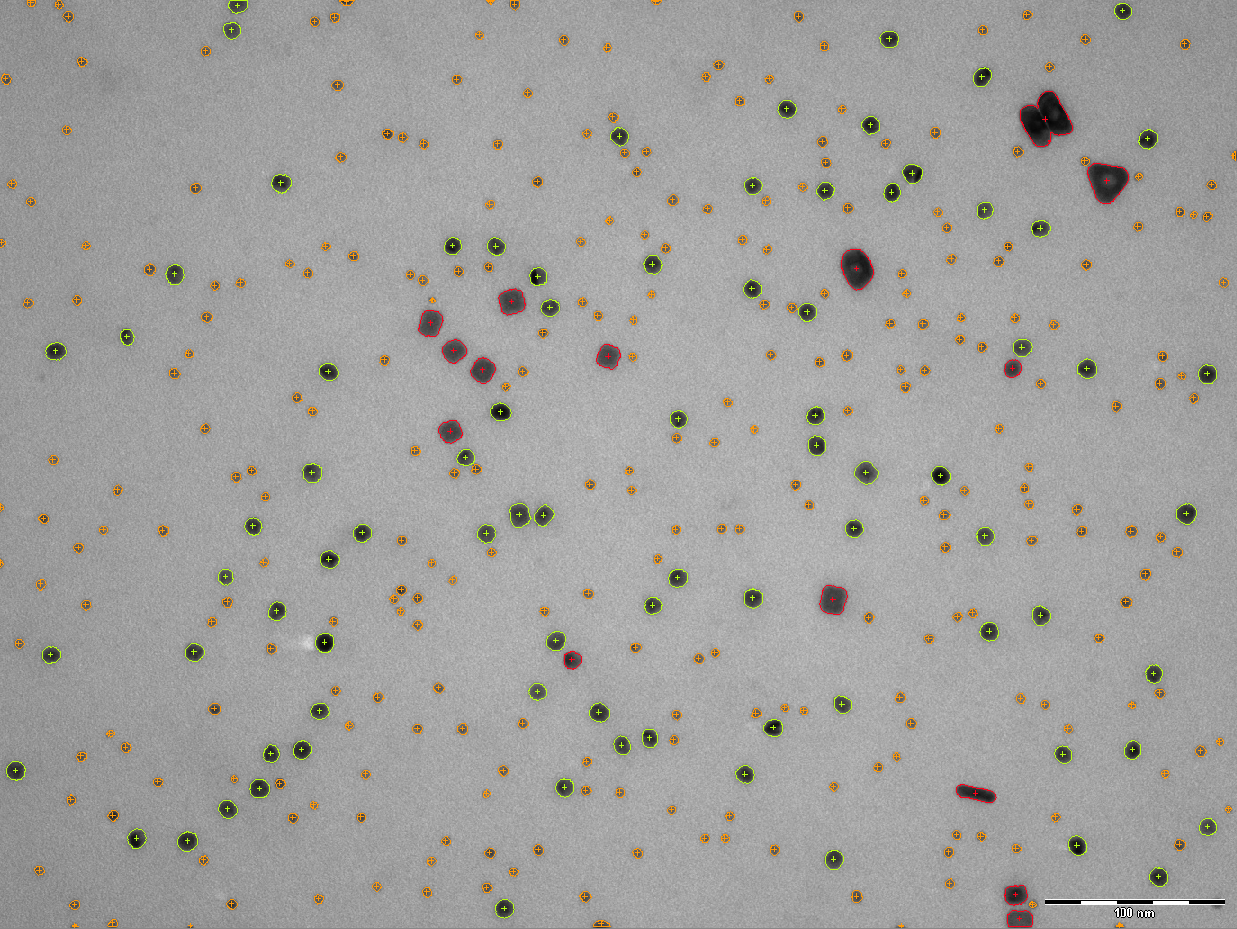
\includegraphics[width=\textwidth]{figures/multi2_klasifikace.png}
\label{fig:class2}
\caption{Výsledek klasifikace částic pro vzorek 2.}
\end{figure}

\begin{table}[h]
\begin{center}
\begin{tabular}{lllll}
\rowcolor[HTML]{9B9B9B} 
\multicolumn{1}{|l|}{\cellcolor[HTML]{9B9B9B}Třída} & \multicolumn{1}{l|}{\cellcolor[HTML]{9B9B9B}Dobře} & \multicolumn{1}{l|}{\cellcolor[HTML]{9B9B9B}Špatně}  & \multicolumn{1}{l|}{\cellcolor[HTML]{9B9B9B}Celkem} & \multicolumn{1}{l|}{\cellcolor[HTML]{9B9B9B}Přesnost} \\ \hline
\multicolumn{1}{|l|}{}                              & \multicolumn{1}{l|}{0}                             & \multicolumn{1}{l|}{2}                               & \multicolumn{1}{l|}{2}                              & \multicolumn{1}{l|}{0,000}                            \\ \hline
\multicolumn{1}{|l|}{}                              & \multicolumn{1}{l|}{2}                             & \multicolumn{1}{l|}{0}                               & \multicolumn{1}{l|}{2}                              & \multicolumn{1}{l|}{100,000}                          \\ \hline
\multicolumn{1}{|l|}{}                              & \multicolumn{1}{l|}{267}                           & \multicolumn{1}{l|}{0}                               & \multicolumn{1}{l|}{267}                            & \multicolumn{1}{l|}{100,000}                          \\ \hline
\multicolumn{1}{|l|}{}                              & \multicolumn{1}{l|}{72}                            & \multicolumn{1}{l|}{11}                              & \multicolumn{1}{l|}{83}                             & \multicolumn{1}{l|}{86,747}                           \\ \hline
\multicolumn{1}{|l|}{Celkem}                        & \multicolumn{1}{l|}{341}                           & \multicolumn{1}{l|}{11}                              & \multicolumn{1}{l|}{352}                            & \multicolumn{1}{l|}{96,875}                           \\ \hline
\end{tabular}
\end{center}
\caption{Vyhodnocení klasifikace částic pro vzorek 2.}
\label{tab:classresult2}
\end{table}

\newpage
\FloatBarrier
\subsection{Vzorek 3}
V této části se nachází zjištěné hodnoty výsledků klasifikace pro vzorek 3.

\begin{figure}[h]
\center
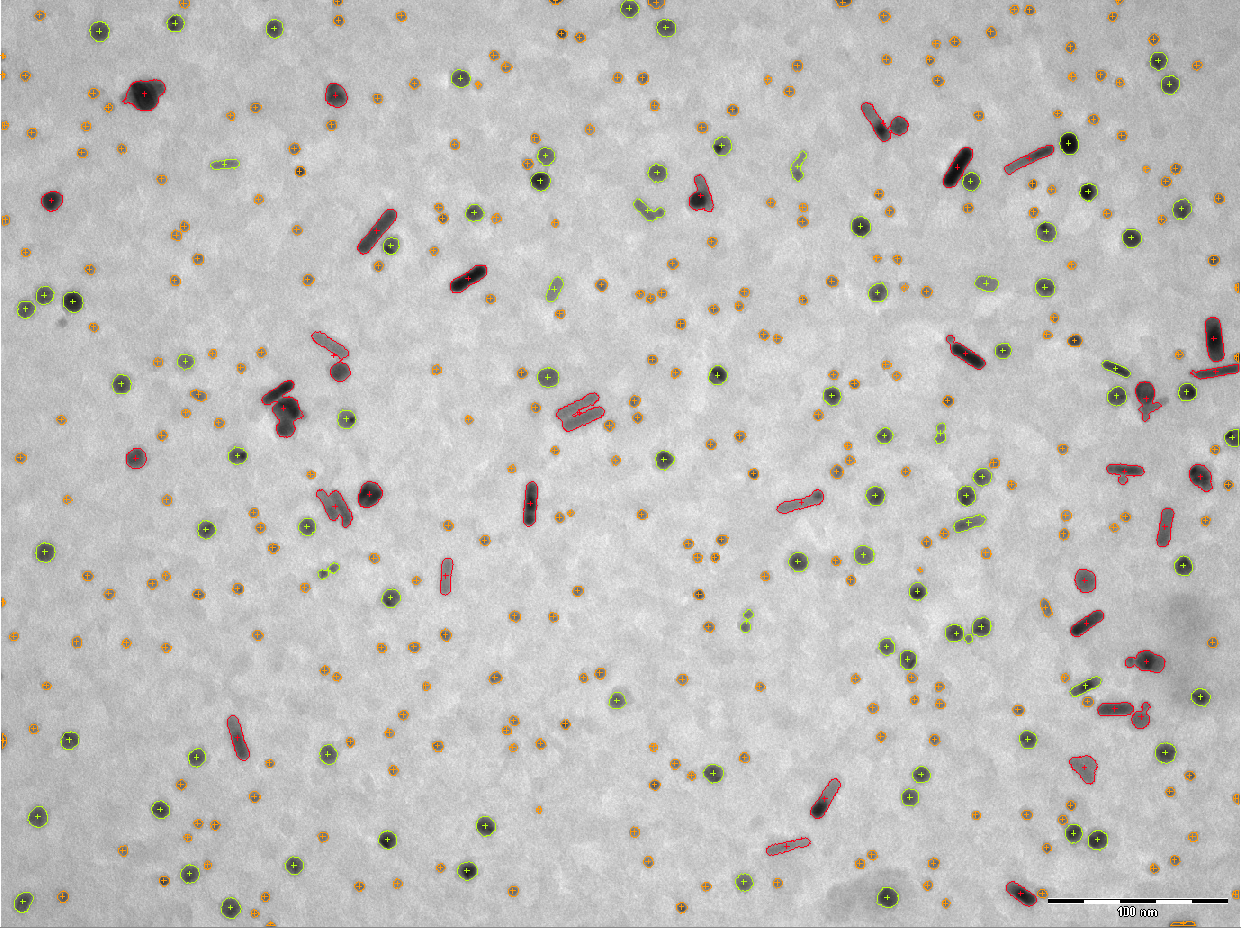
\includegraphics[width=\textwidth]{figures/multi4_klasifikace.png}
\label{fig:class3}
\caption{Výsledek klasifikace částic pro vzorek 3.}
\end{figure}

\begin{table}[h]
\begin{center}
\begin{tabular}{lllll}
\rowcolor[HTML]{9B9B9B} 
\multicolumn{1}{|l|}{\cellcolor[HTML]{9B9B9B}Třída} & \multicolumn{1}{l|}{\cellcolor[HTML]{9B9B9B}Dobře} & \multicolumn{1}{l|}{\cellcolor[HTML]{9B9B9B}Špatně}  & \multicolumn{1}{l|}{\cellcolor[HTML]{9B9B9B}Celkem} & \multicolumn{1}{l|}{\cellcolor[HTML]{9B9B9B}Přesnost} \\ \hline
\multicolumn{1}{|l|}{-1}                            & \multicolumn{1}{l|}{0}                             & \multicolumn{1}{l|}{5}                               & \multicolumn{1}{l|}{2}                              & \multicolumn{1}{l|}{0,000}                            \\ \hline
\multicolumn{1}{|l|}{0}                             & \multicolumn{1}{l|}{20}                            & \multicolumn{1}{l|}{2}                               & \multicolumn{1}{l|}{22}                             & \multicolumn{1}{l|}{90,909}                           \\ \hline
\multicolumn{1}{|l|}{1}                             & \multicolumn{1}{l|}{296}                           & \multicolumn{1}{l|}{0}                               & \multicolumn{1}{l|}{296}                            & \multicolumn{1}{l|}{100,000}                          \\ \hline
\multicolumn{1}{|l|}{2}                             & \multicolumn{1}{l|}{86}                            & \multicolumn{1}{l|}{10}                              & \multicolumn{1}{l|}{96}                             & \multicolumn{1}{l|}{89,583}                           \\ \hline
\multicolumn{1}{|l|}{Celkem}                        & \multicolumn{1}{l|}{402}                           & \multicolumn{1}{l|}{12}                              & \multicolumn{1}{l|}{414}                            & \multicolumn{1}{l|}{97,101}                           \\ \hline
\end{tabular}
\end{center}
\caption{Vyhodnocení klasifikace částic pro vzorek 3.}
\label{tab:classresult3}
\end{table}

\newpage
\FloatBarrier
\subsection{Vzorek 4}
V této části se nachází zjištěné hodnoty výsledků klasifikace pro vzorek 4.

\begin{figure}[hb]
\center
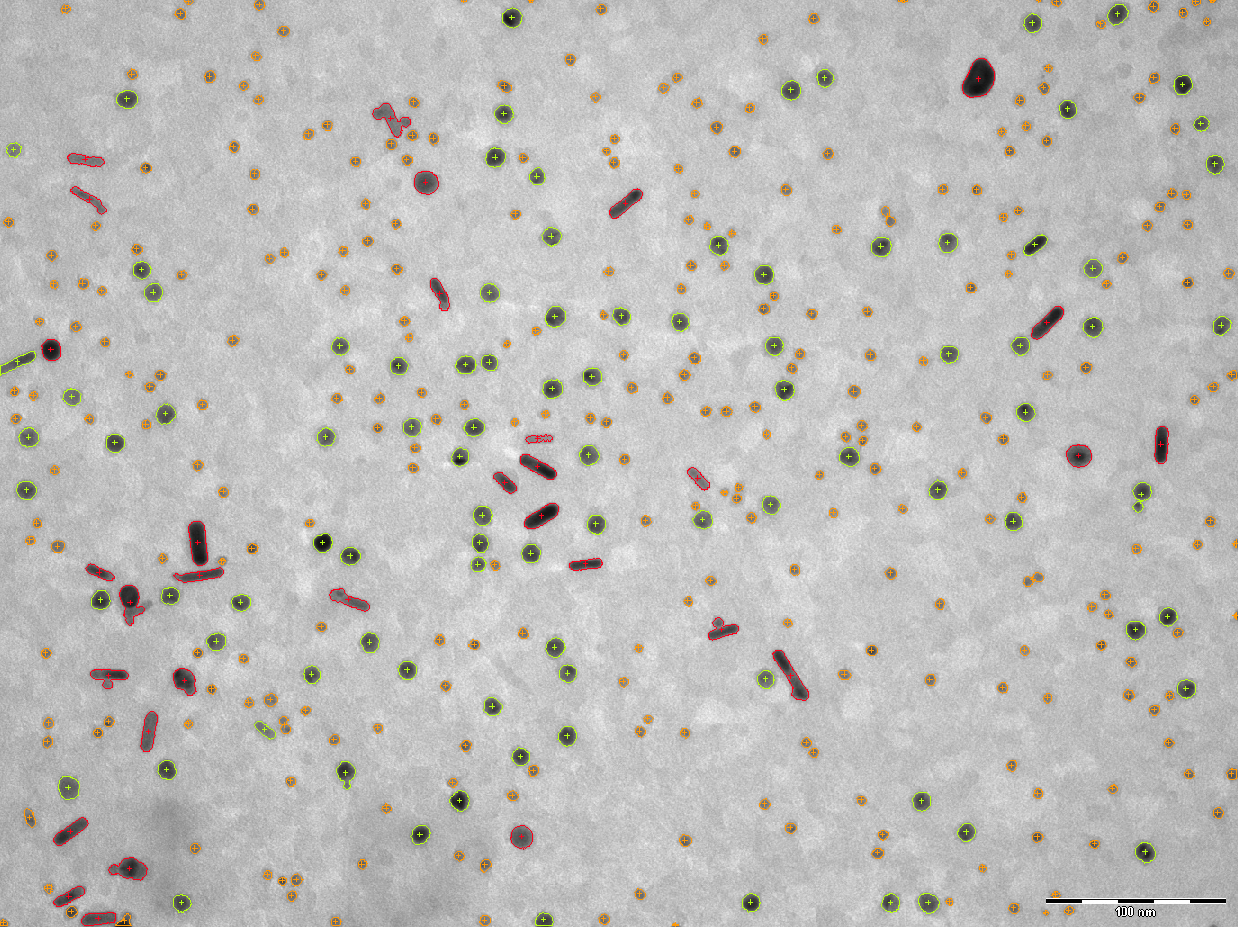
\includegraphics[width=\textwidth]{figures/multi6_klasifikace.png}
\label{fig:class4}
\caption{Vyhodnocení klasifikace částic pro vzorek 4.}
\end{figure}

\begin{table}[h]
\begin{center}
\begin{tabular}{lllll}
\rowcolor[HTML]{9B9B9B} 
\multicolumn{1}{|l|}{\cellcolor[HTML]{9B9B9B}Třída} & \multicolumn{1}{l|}{\cellcolor[HTML]{9B9B9B}Dobře} & \multicolumn{1}{l|}{\cellcolor[HTML]{9B9B9B}Špatně}  & \multicolumn{1}{l|}{\cellcolor[HTML]{9B9B9B}Celkem} & \multicolumn{1}{l|}{\cellcolor[HTML]{9B9B9B}Přesnost} \\ \hline
\multicolumn{1}{|l|}{-1}                            & \multicolumn{1}{l|}{0}                             & \multicolumn{1}{l|}{3}                               & \multicolumn{1}{l|}{2}                              & \multicolumn{1}{l|}{0,000}                            \\ \hline
\multicolumn{1}{|l|}{0}                             & \multicolumn{1}{l|}{17}                            & \multicolumn{1}{l|}{3}                               & \multicolumn{1}{l|}{20}                             & \multicolumn{1}{l|}{85,000}                           \\ \hline
\multicolumn{1}{|l|}{1}                             & \multicolumn{1}{l|}{289}                           & \multicolumn{1}{l|}{2}                               & \multicolumn{1}{l|}{291}                            & \multicolumn{1}{l|}{99,313}                           \\ \hline
\multicolumn{1}{|l|}{2}                             & \multicolumn{1}{l|}{93}                            & \multicolumn{1}{l|}{9}                               & \multicolumn{1}{l|}{102}                            & \multicolumn{1}{l|}{91,176}                           \\ \hline
\multicolumn{1}{|l|}{Celkem}                        & \multicolumn{1}{l|}{399}                           & \multicolumn{1}{l|}{14}                              & \multicolumn{1}{l|}{413}                            & \multicolumn{1}{l|}{96,610}                           \\ \hline
\end{tabular}
\end{center}
\caption{Vyhodnocení klasifikace částic pro vzorek 4.}
\label{tab:classresult5}
\end{table}

\newpage
\FloatBarrier
\subsection{Vzorek 5}
V této části se nachází zjištěné hodnoty výsledků klasifikace pro vzorek 5.

\begin{figure}[h]
\center
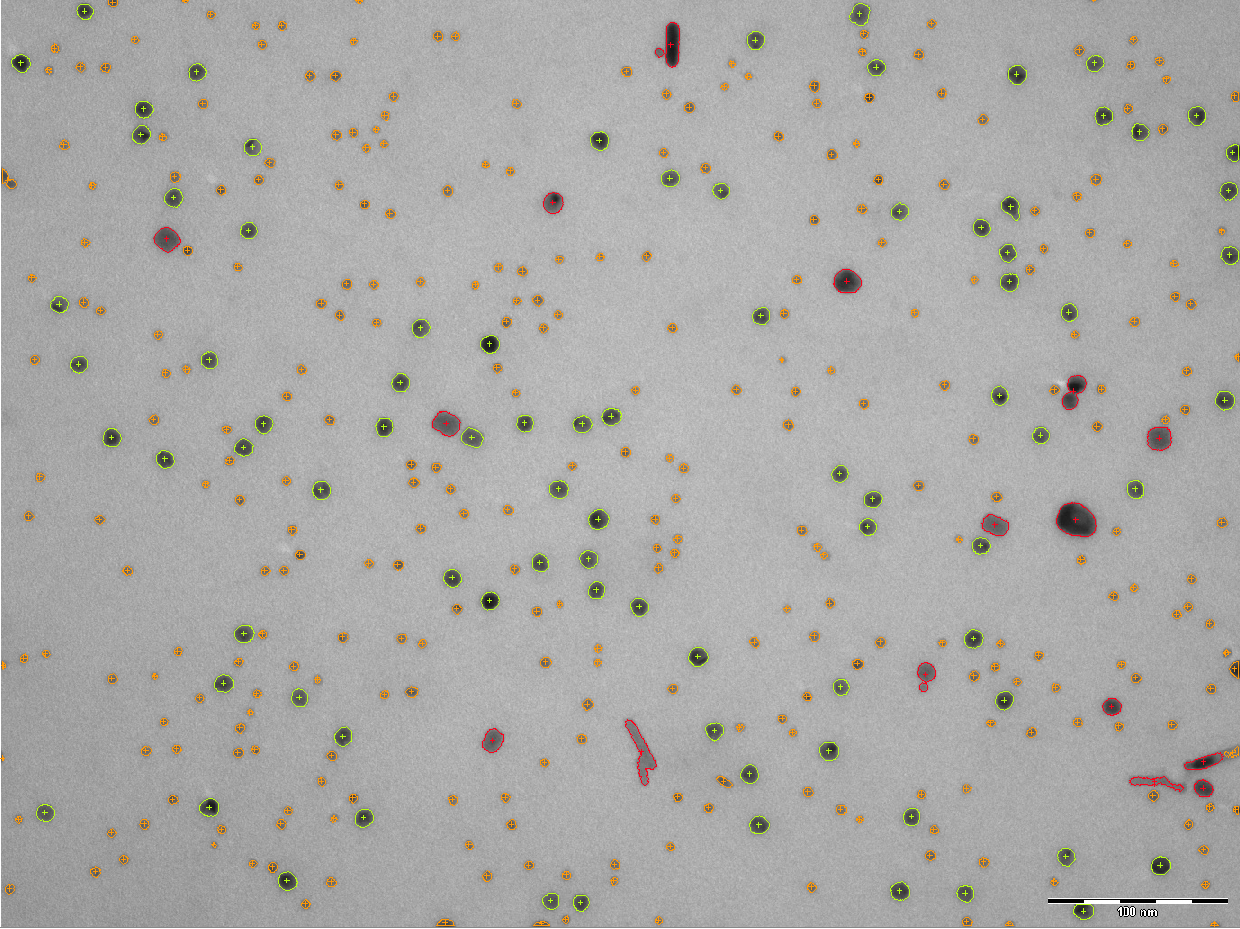
\includegraphics[width=\textwidth]{figures/multi7_klasifikace.png}
\label{fig:class5}
\caption{Výsledek klasifikace částic pro vzorek 5.}
\end{figure}

\begin{table}[h]
\begin{center}
\begin{tabular}{lllll}
\rowcolor[HTML]{9B9B9B} 
\multicolumn{1}{|l|}{\cellcolor[HTML]{9B9B9B}Třída} & \multicolumn{1}{l|}{\cellcolor[HTML]{9B9B9B}Dobře} & \multicolumn{1}{l|}{\cellcolor[HTML]{9B9B9B}Špatně}  & \multicolumn{1}{l|}{\cellcolor[HTML]{9B9B9B}Celkem} & \multicolumn{1}{l|}{\cellcolor[HTML]{9B9B9B}Přesnost} \\ \hline
\multicolumn{1}{|l|}{-1}                            & \multicolumn{1}{l|}{0}                             & \multicolumn{1}{l|}{3}                               & \multicolumn{1}{l|}{2}                              & \multicolumn{1}{l|}{0,000}                            \\ \hline
\multicolumn{1}{|l|}{0}                             & \multicolumn{1}{l|}{4}                             & \multicolumn{1}{l|}{0}                               & \multicolumn{1}{l|}{4}                              & \multicolumn{1}{l|}{100,000}                          \\ \hline
\multicolumn{1}{|l|}{1}                             & \multicolumn{1}{l|}{307}                           & \multicolumn{1}{l|}{0}                               & \multicolumn{1}{l|}{307}                            & \multicolumn{1}{l|}{100,000}                          \\ \hline
\multicolumn{1}{|l|}{2}                             & \multicolumn{1}{l|}{85}                            & \multicolumn{1}{l|}{9}                               & \multicolumn{1}{l|}{94}                             & \multicolumn{1}{l|}{90,426}                           \\ \hline
\multicolumn{1}{|l|}{Celkem}                        & \multicolumn{1}{l|}{396}                           & \multicolumn{1}{l|}{9}                               & \multicolumn{1}{l|}{405}                            & \multicolumn{1}{l|}{97,778}                           \\ \hline
\end{tabular}
\end{center}
\caption{Vyhodnocení klasifikace částic pro vzorek 5.}
\label{tab:classresult6}
\end{table}

\newpage
\FloatBarrier
\subsection{Vzorek 6}
V této části se nachází zjištěné hodnoty výsledků klasifikace pro vzorek 6.

\begin{figure}[h]
\center
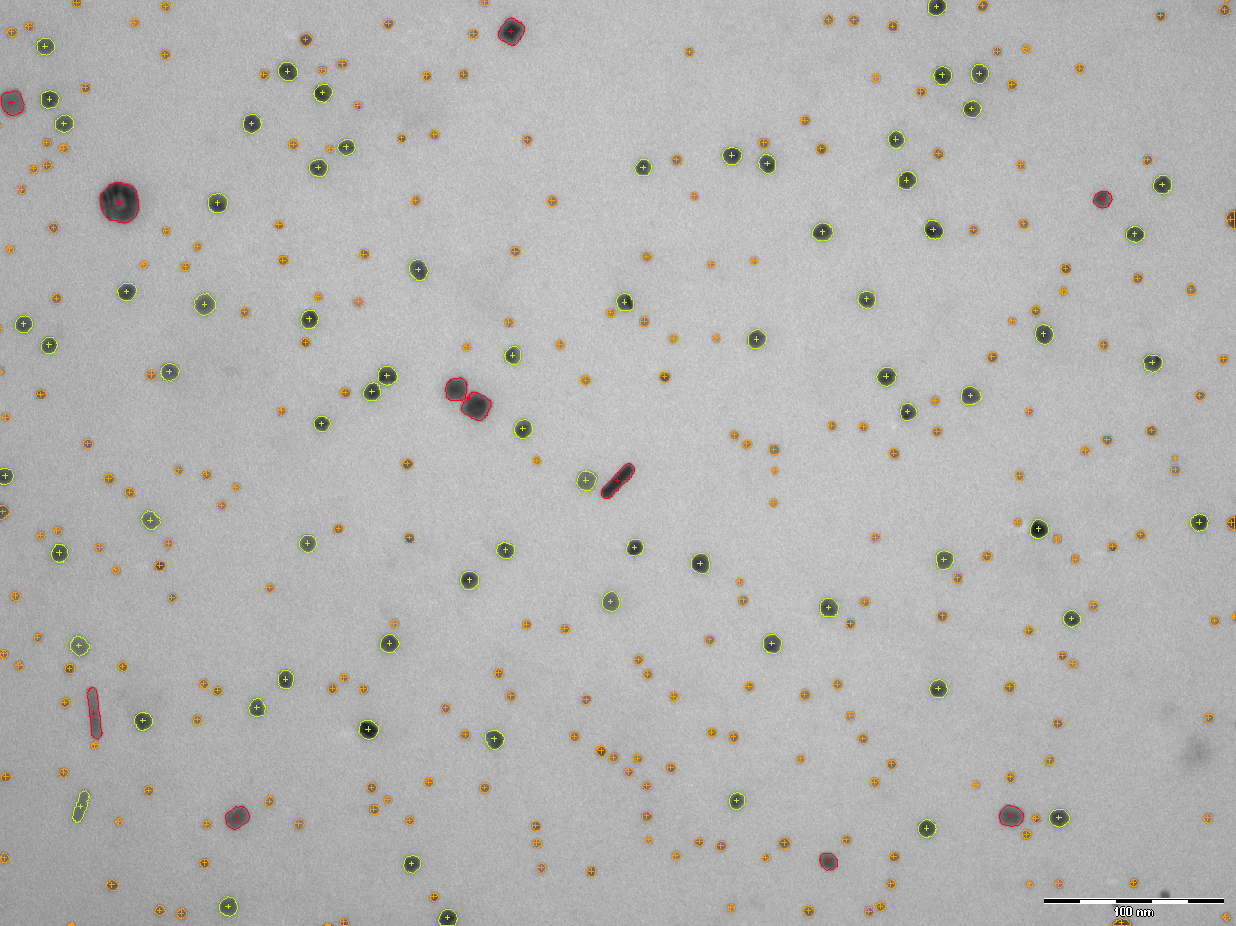
\includegraphics[width=\textwidth]{figures/multi8_klasifikace.png}
\label{fig:class6}
\caption{Výsledek klasifikace částic pro vzorek 6.}
\end{figure}

\begin{table}[h]
\begin{center}
\begin{tabular}{lllll}
\rowcolor[HTML]{9B9B9B} 
\multicolumn{1}{|l|}{\cellcolor[HTML]{9B9B9B}Třída} & \multicolumn{1}{l|}{\cellcolor[HTML]{9B9B9B}Dobře} & \multicolumn{1}{l|}{\cellcolor[HTML]{9B9B9B}Špatně}  & \multicolumn{1}{l|}{\cellcolor[HTML]{9B9B9B}Celkem} & \multicolumn{1}{l|}{\cellcolor[HTML]{9B9B9B}Přesnost} \\ \hline
\multicolumn{1}{|l|}{-1}                            & \multicolumn{1}{l|}{0}                             & \multicolumn{1}{l|}{2}                               & \multicolumn{1}{l|}{2}                              & \multicolumn{1}{l|}{0,000}                            \\ \hline
\multicolumn{1}{|l|}{0}                             & \multicolumn{1}{l|}{2}                             & \multicolumn{1}{l|}{1}                               & \multicolumn{1}{l|}{3}                              & \multicolumn{1}{l|}{66,667}                           \\ \hline
\multicolumn{1}{|l|}{1}                             & \multicolumn{1}{l|}{254}                           & \multicolumn{1}{l|}{0}                               & \multicolumn{1}{l|}{254}                            & \multicolumn{1}{l|}{100,000}                          \\ \hline
\multicolumn{1}{|l|}{2}                             & \multicolumn{1}{l|}{74}                            & \multicolumn{1}{l|}{4}                               & \multicolumn{1}{l|}{78}                             & \multicolumn{1}{l|}{94,872}                           \\ \hline
\multicolumn{1}{|l|}{Celkem}                        & \multicolumn{1}{l|}{330}                           & \multicolumn{1}{l|}{5}                               & \multicolumn{1}{l|}{335}                            & \multicolumn{1}{l|}{98,507}                           \\ \hline
\end{tabular}
\end{center}
\caption{Vyhodnocení klasifikace částice pro vzorek 6.}
\label{tab:classresult7}
\end{table}

\newpage
\FloatBarrier
\subsection{Celkový přehled}
V této části se nachází shrnutí výsledků pro všechny klasifikované vzorky.

\begin{table}[h]
\begin{center}
\begin{tabular}{lllll}
\rowcolor[HTML]{9B9B9B} 
\multicolumn{1}{|l|}{\cellcolor[HTML]{9B9B9B}Třída} & \multicolumn{1}{l|}{\cellcolor[HTML]{9B9B9B}Dobře} & \multicolumn{1}{l|}{\cellcolor[HTML]{9B9B9B}Špatně}  & \multicolumn{1}{l|}{\cellcolor[HTML]{9B9B9B}Celkem} & \multicolumn{1}{l|}{\cellcolor[HTML]{9B9B9B}Přesnost} \\ \hline
\multicolumn{1}{|l|}{-1}                            & \multicolumn{1}{l|}{0}                             & \multicolumn{1}{l|}{22}                              & \multicolumn{1}{l|}{14}                             & \multicolumn{1}{l|}{0,000}                            \\ \hline
\multicolumn{1}{|l|}{0}                             & \multicolumn{1}{l|}{73}                            & \multicolumn{1}{l|}{12}                              & \multicolumn{1}{l|}{85}                             & \multicolumn{1}{l|}{85,882}                           \\ \hline
\multicolumn{1}{|l|}{1}                             & \multicolumn{1}{l|}{1983}                          & \multicolumn{1}{l|}{2}                               & \multicolumn{1}{l|}{1985}                           & \multicolumn{1}{l|}{99,899}                           \\ \hline
\multicolumn{1}{|l|}{2}                             & \multicolumn{1}{l|}{570}                           & \multicolumn{1}{l|}{64}                              & \multicolumn{1}{l|}{634}                            & \multicolumn{1}{l|}{89,905}                           \\ \hline
Celkem                                              & 2626                                               & 100                                                  & 2718                                                & 96,615                                                \\ \hline
\end{tabular}
\end{center}
\caption{Vyhodnocení klasifikace pro všechny vzorky. }
\label{tab:classresult8}
\end{table}

\chapter{Návrh a realizace aplikace}
Tato kapitola popisuje návrh aplikace.

\section{Způsob práce s daty}
Zpracování mikroskopických snímků v laboratoři probíhá typicky po dávkách. Za tímto účelem bylo navrženo rozhraní  které umožňuje seskupovat snímky do skupin. Tyto skupiny nazýváme v aplikaci \textit{Projekty}. Projekt je stromová struktura složek obsahující soubory se snímky a uloženými daty. Více o projektech je uvedeno v sekci o uchování dat \ref{sec:uchovani_dat}.

Typický způsob práce s aplikací je předpokládán následujícím způsobem:
\begin{enumerate}
\item Pořízení skupiny snímků.
\item Vytvoření projektu a načtení skupiny obrázků.
\item Detekce částic ve vybraném obrázku.
\item Možná úprava parametrů detektoru při špatně provedené detekci a opětovná detekce
\item Ruční označení vybraného počtu částic.
\item Přiřazení označených částic klasifikátoru jako trénovací množinu.
\item Klasifikace dosud neoznačených částic natrénovaným klasifikátorem.
\item Oprava nebo trénovací množiny dat.
\item Aplikace detekce a klasifikace na další snímky 
\item Analýza snímků s částicemi.
\end{enumerate}

\section{Uspořádání aplikace}

\begin{figure}
\centering
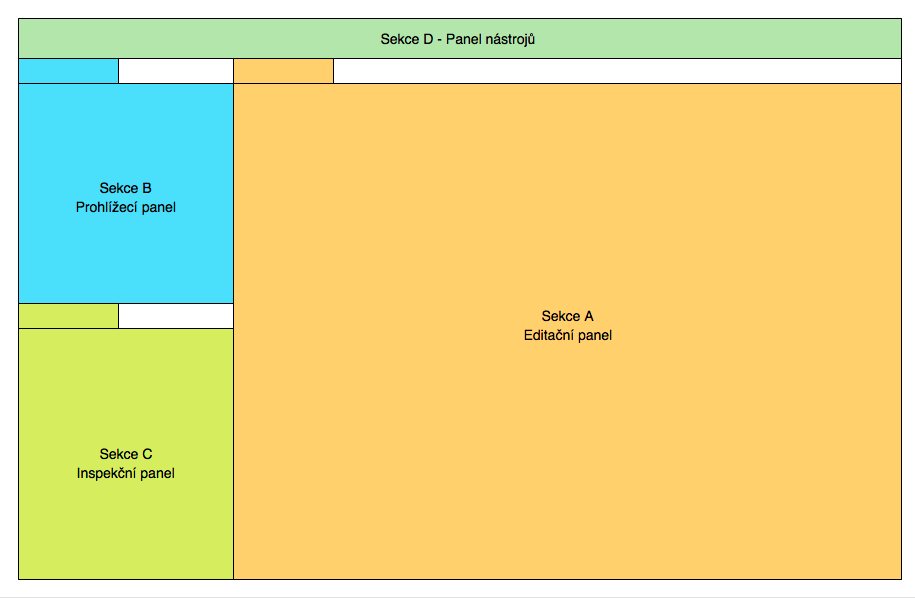
\includegraphics[scale=0.5]{figures/app_overview.png}
\caption{Přehled rozložení aplikace.}
\label{fig:app_overview}
\end{figure}

Na základě těchto požadavků bylo navrženo rozložení aplikace viz.~\ref{fig:app_overview}. 

Hlavní části okna aplikace se skládají z následujících částí:
\begin{description}
	\item[Sekce A - Hlavní editační panel] \hfill \\
	Hlavní editační panel je standardně umístěn uprostřed aplikačního okna a zastává jeho největší část. Panel je určen k zobrazování hlavního obsahu aplikace jako jsou mikroskopické obrázky a analýzy. Jednotlivé položky je možné zobrazit v záložkách. 
	\item[Sekce B - Prohlížecí panel] \hfill \\
	Prohlížecí panel je standardně umístěn v horní levé části aplikačního okna. Komponenty zobrazují jednotlivé projekty a klasifikátory.
	\item[Sekce C - Inspekční panel] \hfill \\
	Inspekční panel je standardně umístěn v dolní levé části hlavního okna. Slouží k zobrazování doplňkových informací o mikroskopickém obrázku nebo o datech v něm umístěných.
	\item[Sekce D - Panel nástrojů] \hfill \\
	Panel nástrojů je umístěn v horní části okna aplikace. Obsahuje kontrolní prvky pro manipulaci s daty v aplikaci.
\end{description}
\subsection{Editační panel}
V editačním panelu je zobrazen buď \textit{editor snímků} nebo \textit{panel analýzy}. 

\subsubsection{Editor snímků}
Editor snímků je hlavní a nejdůležitější součást aplikace. Slouží primárně k práci obrazovými daty jako je detekce a klasifikace. Hlavní funkcí panelu je zobrazování obrazových dat a nanočástic.

Ten umožňuje práci ve třech režimech.
\begin{itemize}
\item výběr
\item značení
\item tvoření
\end{itemize}

První režim \textit{výběr}, je určený k interaktivnímu výběru detekovaných částic. To umožňuje uživateli jak interaktivně zkoumat data tak opravit výsledky detekce.

Druhý režim \textit{značení}, je určený k přiřazování částic do jednotlivých tříd. V tomto režimu uživatel buď poskytuje trénovací data pro klasifikátor, aplikuje klasifikátor na aktuálně zobrazené nanočástice nebo může upravovat výsledek klasifikace.

Třetí režim \textit{tvoření} umožňuje manuální přidávání částic. Tento režim umožňuje umístit novou částici na libovolné místo v obraze.

Nedílnou součástí editace částic je jejich vizualizace. Vizualizace částic realizována přímo pomocí Java 2D Graphics. Jednotlivé částice jsou zobrazovány na obrazovém podkladě. Zobrazení lze přibližovat, oddalovat a volit různé režimy zobrazení částic.

Částice je možné zobrazovat s/bez obrysu a s/bez zobrazeného středu.

\subsubsection{Panel analýzy}
Panel analýzy umožňuje analyzovat data pomocí hierarchického shlukování a výsledek vizualizovat pomocí dendrogramu.

Hierarchické shlukování je sekvence vnořených rozkladů, která na jedné straně začíná triviálním rozkladem, kdy každý objekt dané množiny objektů tvoří jednoprvkový shluk, a na
druhé straně končí triviálním rozkladem s jedním shlukem obsahujícím všechny objekty.
Podle směru postupu při shlukování dělíme metody hierarchického shlukování na aglomerační
a divizivní \cite{on:shlukovani}.

Dendrogram je binární strom znázorňující hierarchické shlukování. V aplikaci je dendrogram vizualizován tak, že každý uzel tohoto stromu představuje shluk. Vertikální řezy dendrogramem jsou rozklady ze shlukovací sekvence. Horizontální směr v dendrogramu představuje vzdálenost mezi shluky (rozklady).

Dendrogramem ve možné vést řezy danou vzdáleností, které rozdělí dendrogram na dílčí shluky. V tomto rozdělení je každý shluk barevně oddělen. Výsledek vzniklého rozdělení má pak uživatel možnost sledovat v původním snímku v NP, kde každá NP má barvu podle příslušnosti do shluku.  

Implementace konstrukce dendrogramu vychází z \cite{on:shlukovani_java}. Původní řešení je modifikováno pro účely aplikace. Byla přidána funkcionalita tvorby řezů v histogramu a upravena vizualizace histogramu.

Ukázka pa

\subsection{Přehled projektů}
\begin{figure}[h]
\centering
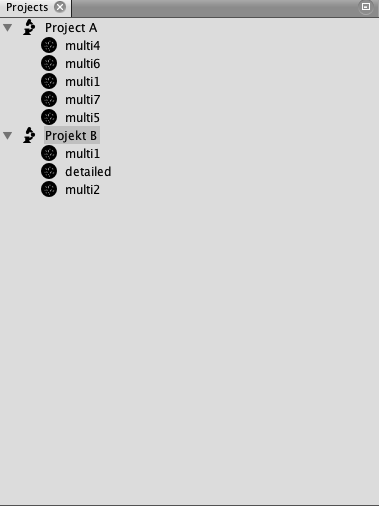
\includegraphics[scale=0.5]{figures/app_project_overview.png}
\caption{Ukázka panelu přehledem projektů a snímků.}
\end{figure}

Přehled otevřených projektů je zobrazen na panelu přehledu projektů. Panel poskytuje uživateli přehled o otevřených projektech a obrázcích v přehledné stromové struktuře. Kořen stromu tvoří projekt. Listy projektu pak znázorňují jednotlivé snímky přiřazené k projektu. Panel je také zodpovědný o přiřazování jednotlivých snímků k projektu a jejich ukládání jednotlivých obrázků.

\subsection{Přehledu klasifikátorů}
\begin{figure}[h]
	\centering
	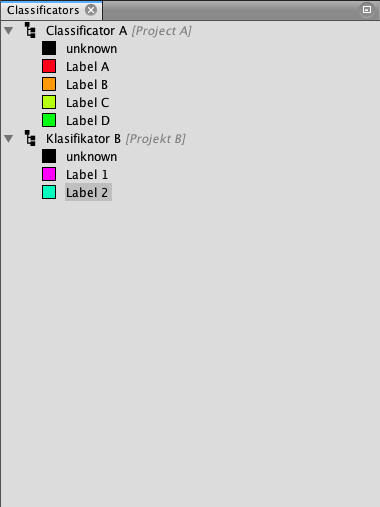
\includegraphics[scale=0.5]{figures/app_class_overview.png}
	\caption{Ukázka panelu s přehledem klasifikátorů.}
\end{figure}

Panel klasifikátoru je standardně součástí prohlížecího panelu. Jeho funkcí je zobrazovat vytvořené klasifikátory, vytvářet klasifikátory nové a poskytovat uživateli možnost s klasifikátorem manipulovat.

Klasifikátoru lze vytvořit jednotlivé třídy pro zařazení částic. Každou třídu je možné pojmenovat a přiřadit k ní barvu. Přiřazená barva klasifikátoru ovlivňuje jakou barvou jsou částice, přiřazené do dané třídy, zobrazovány v \textit{editoru obrázků}.

Klasifikátor je možné exportovat, importovat a tím přenášet mezi jednotlivými projekty.

\subsection{Inspekční panel}
Inspekční panel obsahuje v základní verzi dva panely. Panel s informacemi o snímku a inspekční panel.

Panel s \textbf{informacemi o snímku} zobrazuje uživateli obecné informace o snímku jako je jeho rozlišení, absolutní počet detekovaných částic, počet částic v jednotlivých třídách atd. Ukázka panelu je zobrazena na obr.~\ref{fig:app_image_info}.

\begin{figure}[h]
	\centering
	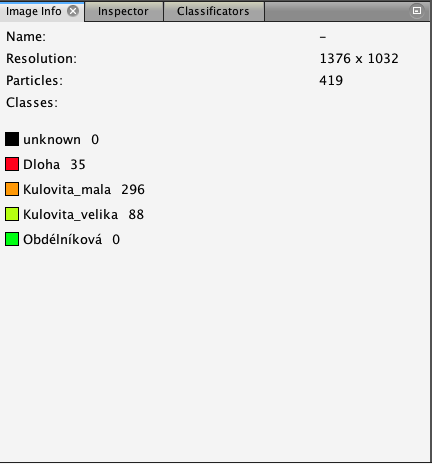
\includegraphics[scale=0.5]{figures/app_image_info.png}
	\caption{Ukázka panelu s informacemi o snímku.}
	\label{fig:app_image_info}
\end{figure}

\textbf{Inspekční panel} zobrazuje informace o částicích které má uživatel vybrané. Takovou informací je např. počet vybraných částic, příslušnost částic do tříd, těžiště atd. Vybrané částice je pak možné exportovat do textového formátu CSV k další analýze. Ukázku panelu je možné pozorovat na obr.~\ref{fig:app_inspector}.

\begin{figure}[h]
	\centering
	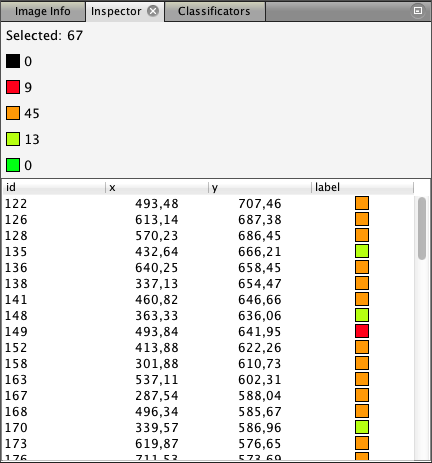
\includegraphics[scale=0.5]{figures/app_inspector.png}
	\caption{Ukázka panelu s informacemi o snímku.}
	\label{fig:app_inspector}
\end{figure}

\section{Uchování dat}
\label{sec:uchovani_dat}
Pro uchovávání dat je v aplikaci navržena struktura složek a souborů nazvaná \textit{projekt}. Struktura projektu se sestává ze tří složek, souboru \textit{pattern.proj} a souborů s daty viz obr.~\ref{fig:project_structure}.

\begin{figure}
	\centering
	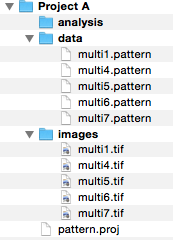
\includegraphics[scale=1]{figures/app_project_structure.png}
	\caption{Příklad souborové a složkové struktury projektu.}
	\label{fig:project_structure}
\end{figure}

Aplikace umožňuje uchovávat:
\begin{itemize}
\item pro každý snímek informace o detekovaných a klasifikovaných hodnotách NP.
\item informace o klasifikátoru projektu
\end{itemize}

\subsubsection{Ukládání dat snímků}
Data pro jednotlivé snímky jsou uchovávány ve složce \textit{data} v souborech s příponou \textit{.pattern}. Název souboru s daty pak odpovídá názvu souboru snímku ke kterému data patří. Pro ukládání dat je využito formátu JSON \cite{json}. Příklad struktury ukládaného dokumentu je následující:
\begin{lstlisting}[language=json,firstnumber=1]
{
	"name": "multi2",
	"image": "multi2.tif",
	"particles": [
  	{
  	"id": 0,
  	"cog": {
     	"x": 1003.0,
     	"y": 1029.5
   	},
   	"contour": [
     {
     	"x": 1001.0,
     	"y": 1029.0
     },
     {
     	"x": 1001.0,
     	"y": 1030.0
     },
     {
     	"x": 1005.0,
     	"y": 1030.0
     },
     {
     	"x": 1005.0,
     	"y": 1029.0
     }
   ]
}
\end{lstlisting}


\subsubsection{Ukládání dat klasifikátoru}
Data pro klasifikátor se ukládají přímo do souboru \textit{pattern.proj}, který se nachází v kořenovém adresáři projektu. Příklad struktury ukládaných dat ve fromátu JSON
\begin{lstlisting}[language=json,firstnumber=1]
{
  "info": {
    "id": "Classificator A",
    "path": "path/to/pattern.proj"
  },
  "labels": [
    {
      "id": -1,
      "name": "unknown",
      "color": {
        "value": -16777216,
        "falpha": 0.0
      }
    }
    ...
   ]
  "selectedLabel": 2,
  "examples": [
    {
      "id": 47,
      "cog": {
        "x": 841.6866566716642,
        "y": 918.4822588705647
      },
      "contour": [ ... ]
    }
   ]
}
\end{lstlisting}

\section{Realizace aplikace}
Celá aplikace je realizována v prostředí prostřednictvím programovacího jazyka Java pomocí frameworku NetBeans Platform.

\subsection{Vývojové prostředí}
Netbeans Platform je programové prostředí patřící do skupiny Rich Client Platform (RCP). RCP je soubor programátorských nástrojů zjednodušující vývoj aplikace. Většina RCP poskytuje následující funkce:
\begin{itemize}
	\item manažer životního cyklu aplikace
	\item bundling framework
	\item pokročilé nástroje pro tvorbu uživatelského rozhraní
	\item nástroje pro internacionalizaci
	\item 
\end{itemize}

Příklady takových frameworků pro jazyk Java jsou Eclipse RCP, Netbeans Platform a Spring Framework.

\subsubsection{Netbeans Platform}
Pro vývoj aplikace byla zvolena NetBeans platform na základě dřívějších zkušeností autora. NetBeans Platform nabízí ucelenou sadu komponent, podpůrných tříd a propracovanou modulární architekturu s konkrétními promyšlenými API, které výrazně urychlí vývoj a správu programů.

\subsection{Podpůrné knihovny}
V aplikace používá následující dostupné opensource knihovny:
\begin{description}
	\item[OpenCV] Knihovna s funkcemi pro zpracování obrazu, počítačové vidění a strojové učení.
	\item[Bio-formats] Knihovna podporující načítání snímků v rozličných formátech.
	\item[hierarchical-clustering-java] Knihovna s implementací hierarchického shlukování.
	\item[japura-gui] Knihovna s dodatečnými komponentami uživatelského rozhraní.
	\item[gson] Knihovna zjednodušující serializaci a de-serializaci objektů ve formátu JSON.
\end{description}


\chapter{Diskuze}
V této kapitole jsou rozebrány výsledky detekce a klasifikace.

Navržená metoda detekce částic má problémy při separování částic, které jsou příliš blízko u sebe. Takové částice se vyznačují nízkou nebo téměř žádnou magnitudou gradientu v místě přechodu mezi částicemi.

Tento problém jsem se pokoušel velice aktivně řešit, ale žádné zvolené řešení nevedlo k ideální segmentaci. Proběhl pokus o zpřesnění segmentace pomocí metody watershed. Problémem watershedu je, že potřebuje znát počáteční místa ve snímku, odkud může růst. Právě nalezení těchto míst je klíčovou součástí úspěšné segmentace pomocí watershed algoritmu.

Vyzkoušel jsem hledání těchto míst pomocí distanční transformace i iterativní eroze na nekonvexní objekty. Konvexita se projevila být dobrým testem pro špatně nebo dobře segmentované částice. Ty špatně segmentované jsou nekonvexní.

Takto aplikovaný watershed dokázal oddělit některé částice lépe. Avšak na jiných případech vykazoval chybu v podobě přesegmentovaní a negativně ovlivňoval výsledky celé segmentace a následně klasifikace. Proto nakonec jako výsledné řešení bylo ponecháno "pouze primitivní" adaptivní prahování aby nedocházelo ke zbytečné zátěži programových a hardwarových komponent. S tím že případná oprava bude ponechána na interaktivním zásahu uživatele.

Navržený klasifikátor umožňuje klasifikovat data a jeho přesnost byla uznána laboranty jako dostačující. Velikým přínosem je, že klasifikátor dokáže úspěšně klasifikovat částice typu kolečko od zbytku. Jelikož částic typu kolečko se ve snímcích nachází nejvíce a problematicky se trefují pomocí myši, jejich přeznačování by stálo značné úsilí. Takto laborant může přeznačit okolo 10 špatně klasifikovaných částic, které se dobře trefují myší. Tento úkon pak zabírá minimální 

Zhodnocení výsledků detekce. Pořád to není úplně ono navržené metody stále selhávají např. na obr. Důvodem je malý nejčastěji kontrast částic s okolím. Nebo jejich těsná blízkost\\
Zhodnocení výsledků klasifikace. Byl ozkoušeno testování pomocí konvexity ale nepodařilo se dotáhnout do konce.

Implementovaná aplikace byla otestována a funguje na operačních systémech Windows 7/8.1 a Mac OS X 10.9.

Aplikace nyní míří do testovacího provozu, ve kterém se prověří její skutečná funkčnost. Aplikaci chci dále ladit a rozvíjet jako opensource projekt.

\chapter{Závěr}
\section{Shrnutí práce}
Diplomová práce se zabývá problematikou automatizované analýzy nanočástic v mikroskopických snímcích. Je rozebrána důležitost automatizované analýzy nanočástic. Následně jsou uvedeny základní požadavky na program schopný takovou analýzu provádět. Je zjištěno že pro úspěšnou analýzu nanočástic v mikroskopických snímcích je potřeba částice nejprve správně detekovat a následně klasifikovat.

Pro účely detekce jsou nejprve algoritmy které umožňují detekci nanočástic v mikroskopických snímcích. Na základě analýzy je vybrán zvolený způsob detekce nanočástic. Zvolený algoritmus detekce využívá adaptivního prahování a morfologických operací. Algoritmus byl implementován v jazyce Java za využití knihovny OpenCV. Výstupy detekčního algoritmu jsou analyzovány a vyhodnoceny na reálných testovacích datech. Úspěšnost detekce obecně nejde pod 90\%. Zvolený algoritmus má problémy při detekci částic, které se překrývají nebo jsou blízko u sebe.

Dále jsou analyzovány způsoby klasifikace nanočástic v mikroskopických snímcích. Na základě analýzy je vybrán vhodný klasifikační algoritmus. Jako klasifikační algoritmus bylo vybrán algoritmus k-nejbližších sousedů. Jsou uvedeny výsledky klasifikace za použití K-NN na reálných testovacích datech pocházejících z provozu UMG. Úspěšnost klasifikace pomocí K-NN nejde pod 80\%.

Detekční a klasifikační algoritmus je součástí implementovaného programu, který umožňuje automatizovanou detekci, klasifikaci a analýzu nanočástic. Program poskytuje pro analýzu nanočástic rozličné inspeční nástroje jako je shluková analýza pomocí dendrogramu a další. Program je naimplementován v programovacím jazyce jazyce Java za využití frameworku NetBeans Platform.

Výše zmíněné postupy pak vedou k celkovému urychlení procesu analýzy snímků.

\section{Další směřování}
Aplikace nyní míří do testovacího provozu na UMG, kde bude vyhodnocen její přínos. Další možný vývoj na aplikaci se bude skládat z vylepšování uživatelského rozhraní a doplnění o další funkcionalitu, která vyplyne z testovacího provozu.

Detekční a klasifikační algoritmus bude testován v reálném provozu, kde se ověří jeho funkčnost na větším počtu snímku. V případě nefunkčnosti některé částic algoritmu na budoucích datech budou selhání vyhodnocena a algoritmus upraven.

Mikroskopické vzorky se jsou často objemové a snímají se po jednotlivých řezech. Další rozvoj aplikace a algoritmů by pak mohl směřovat na poskytnutí nástrojů pro automatizovanou analýzu nanočástic ve třírozměrném prostoru.

%*****************************************************************************
% Seznam literatury

\bibliographystyle{csplainnat}
{
\bibliography{reference}
}
%*****************************************************************************
\appendix


%*****************************************************************************
\chapter{Seznam použitých zkratek}

\begin{description}
\item[NP] - Nanočástice, z aglického \textit{nanoparticles}
\item[TEM] - Transmisní elektronová mikroskopie
\item[SEM] - Rastrovací elektronový mikroskop
\item[UMG] - Ústav molekulární genetiky, Ústav Akademie Věd České Republiky
\end{description}

%*****************************************************************************
\chapter{Obsah přiloženého CD}
V této kapitole naleznete obsah CD přiloženého k této diplomové práci.

\begin{itemize}
	\item readme.txt - popis obsahu CD s dalšími informacemi
	\item pattern/ - zdrojové kódy aplikace v jazyce Java
	\item text/
	\begin{itemize}
		\item src/ - zdrojový text v LaTeXu, včetně obrázků a šablon
		\item palasjir\_2015dip.pdf - text diplomové práce ve formátu PDF
	\end{itemize} 
\end{itemize}

\chapter{Snímky obrazovky}
\label{apend:screens}

\begin{figure}
	\centering
	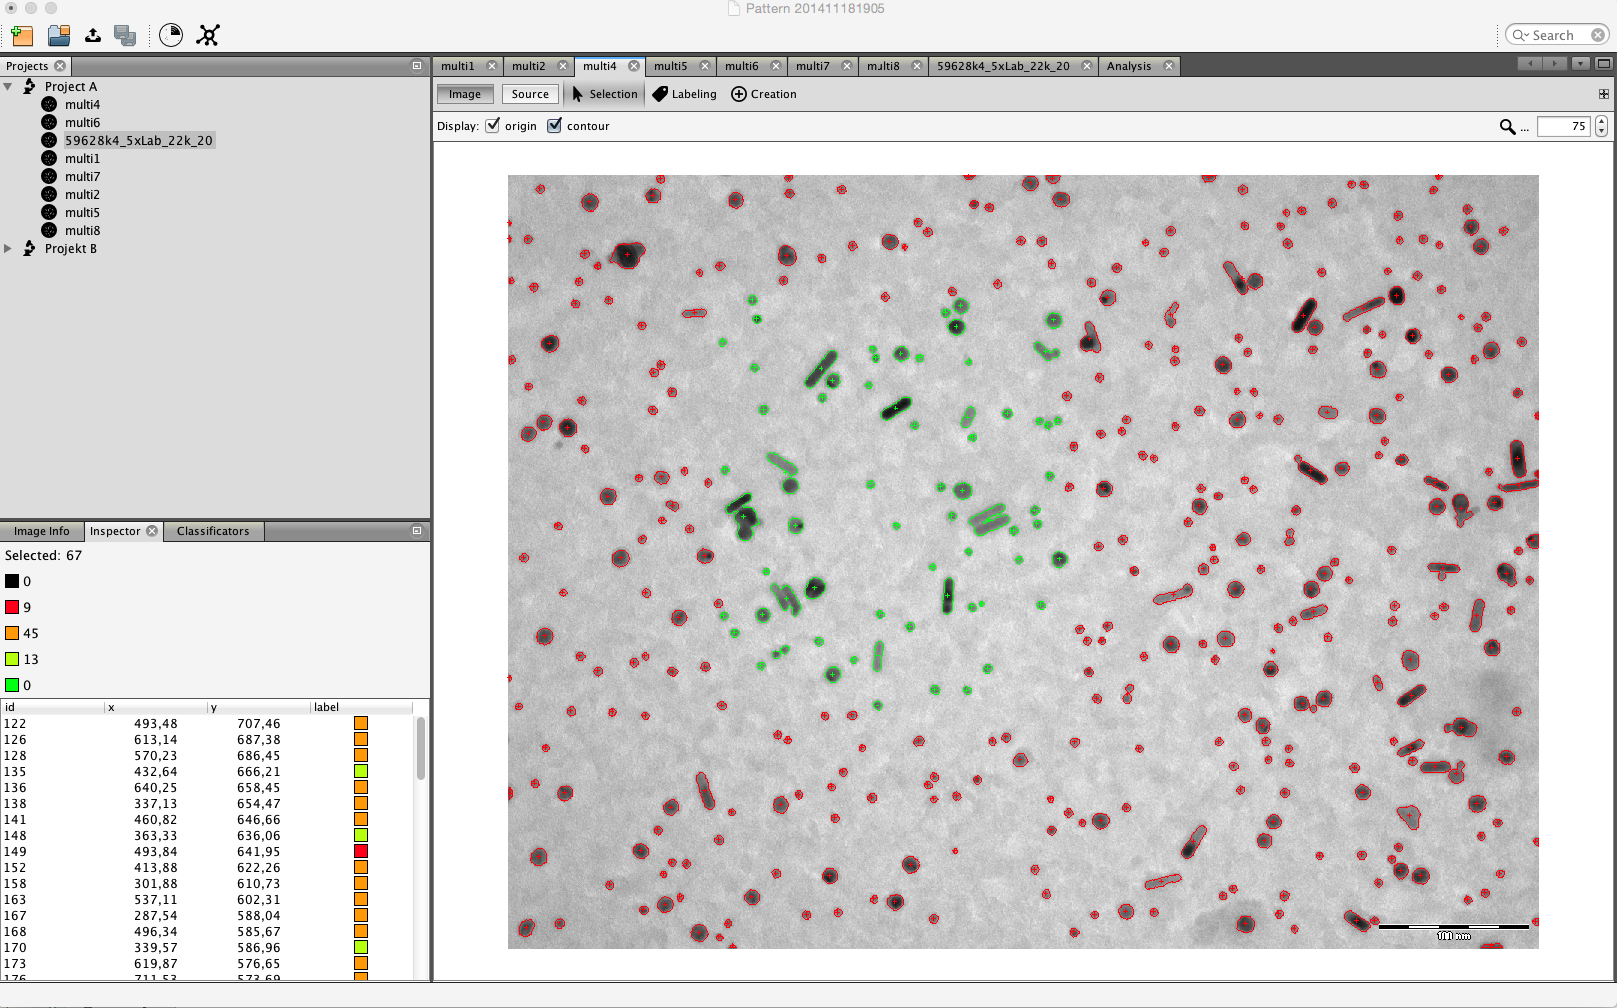
\includegraphics[scale=1]{figures/app_screen_selection.png}
\end{figure}


\end{document}
